\documentclass{article}
\usepackage[utf8]{inputenc}
\usepackage{amsmath}
\usepackage{amssymb}
\usepackage{verbatim}
\usepackage{float}
\usepackage{graphicx}
\usepackage{bbm}
\usepackage{geometry}
\usepackage{subfig}
\title{Investigation of Effect of Location Errors in Synthetic Aperture Radar Image Reconstruction}
\author{Aidan Fitzpatrick \\ Soheil Hor \\ Quint Underwood }
\date{\today}

\begin{document}

\maketitle

\section{Introduction}
\indent \indent
Radar imaging is one of the most well-known imaging technologies that allows for robust and accurate images of different scenes using electromagnetic waves. Traditional radar systems required large antennas that could only be mounted on aircraft, satellites, or ground stations. This largely limited radar imaging to remote sensing and radio astronomy. Recent developments in millimeter-wave radar technology have resulted in radar modules that can fit on a circuit board only a few inches wide and with very high range-resolution. However, in commercial applications like radar guidance of autonomous vehicles and drones the effect of limited aperture size on lateral resolution still remains a main challenge.
\newline
\indent
In this paper, we first describe and analyze the range and azimuth resolution that can be achieved using real aperture radar. We present that range resolution can be sufficient with a single aperture through the use of matched filtering and range modulation techniques; however, the azimuth resolution is poor with the use of a single aperture. This motivates the use of synthetic aperture radar (SAR) to improve resolution in the azimuth direction. We describe the difficulties inherent to SAR reconstruction and then describe a few well-known signal processing-based reconstruction algorithms for this task. We then derive the reconstruction error that results from azimuth-location errors applied to two signal processing reconstruction algorithms. Finally, we complement our analysis with investigation of the effectiveness of neural networks in mitigation of the mentioned azimuth-location errors in mmWave SAR image reconstruction systems.


\section{Radar Imaging Basic}
\indent \indent
In this section we will explain some of the fundamental aspects of radar imaging, none of which are specific to SAR but are nonetheless essential components of deriving any useful results in SAR.  The signal-to-noise ratio (SNR) of a traditional pulsed radar imaging system is dependent on the transmitted pulse energy. In order to achieve high pulse energies, the system typically must employ long pulse widths due to practical limitations on peak power. As pulsed width is increased, range resolution decreases proportionally resulting in a significant design trade-off between resolution and SNR. By implementing signal processing techniques, the performance of radar imaging systems can break the bounds of this trade-off. In this section, we will discuss matched filtering and range modulation techniques that are commonly utilized in radar imaging and serve as the backbone to the reconstruction algorithms provided in Section 4. In addition, we will analyze typical approaches for obtaining better azimuth resolution.

\subsection{Range Resolution}

\subsection*{Matched Filtering}
\indent \indent
We begin with the simplest radar task: estimating the distance to a target along one dimension, which is demonstrated in Figure \ref{range_diagram}. A perfect measurement of the targets would yield a delayed delta function times the radar reflectivity \( \sigma_{n} \) of the targets, which we call the ideal target function:
\begin{displaymath}
	f_0(x) = \sum\limits_{n}^{} \sigma_{n} \delta(x - x_{n})  
\end{displaymath}
We can never achieve this ideal target function because transmitting an impulse response requires infinite bandwitdth. In practice, we image the target with the radar signal \( p(t) \):
\begin{displaymath}
	s(t) = \sum\limits_{n}^{} p(t - \frac{2 xn}{c}) 
\end{displaymath}
where \( 2 x_{n} / c\) is the round-trip delay to the nth target. Therefore, \( x = ct/2 \) and we can write 
\begin{displaymath}
	s(t) = f_0(t) * p(t) = f_0(\frac{ct}{2}) * p(t)  
\end{displaymath}
The above model ignores 1) the inverse square amplitude factor as a function of distance, and 2) the frequency dependency of the target reflectivity.
We can take the Fourier transform of the echoed signal:
\begin{displaymath}
	S(\omega) = P(\omega) \sum\limits_{n}^{} \sigma_{n}exp(-j \omega \frac{2 x_{n}}{c}) 
\end{displaymath}
We want to recover the target information, which can be achieved via matched filtering. We let \( s_{M}(t) \) denote the matched-filtered echoed signal.
\begin{align*}
	s_{M}(t) &= \mathcal{F}^{-1}_{( \omega )} [S(\omega) P^{*}(\omega) ] \\
			 &= \mathcal{F}^{-1} \left[ \sum\limits_{n}^{} \sigma_{n} | P(\omega)^2 | exp\left( -j \omega \frac{2 x_{n}}{c} \right) \right] \\
			 &= \sum\limits_{n}^{} \sigma_{n} \text{psf}_{t} \left(t - \frac{2 x_{n}}{c} \right) 
\end{align*}
And we define the point spread function as
\begin{displaymath}
	\text{psf}_{t}(t) = \mathcal{F}^{-1}_{( \omega )} \left[|P(\omega) |^2 \right]
\end{displaymath}
We also note that as the bandwidth of \( p(t) \) increases, our image becomes sharper:
\begin{align*}
	f(x) &= s_{M}(t) \\
		 &= \sum\limits_{n}^{} \text{psf}_{t} \left[ \frac{2}{c}(x - x_{n}) \right] \\
		 &= f_{0}(x) * \text{psf}(x) 
\end{align*}
This motivates the use of the FM chirp, which we will cover next.



\subsection*{FM Chirps}
\indent \indent
Our ideal radar signal would be a high-bandwidth signal transmitted over a short time window (i.e. a delta function). This is not feasible because of power constraints, so to achieve the necessary bandwidth we can emit a signal that increases in frequency linearly as a function of time. Such a function is known as an FM pulsed chirp signal, and is expressed as
\begin{displaymath}
	p(t) = a(t) exp(j \beta t + j \alpha t^2 )
\end{displaymath}
where \( \alpha(t) =1 \) for \( 0 \leq t \leq T \), and T is the chirp pulse duration. We also note the psf(x) for a chirp signal:
\begin{align*}
	psf(x) &= \mathcal{F}_{(t)} [a^{*}(t) ] \\
\end{align*}
Since \( a(t) \) is a rectangular pulse, the point spread function of an FM chirp is a sinc function. This means that matched filtering of chirp signals in one-dimensional range imaging will result in sinc-like blips indicating a target. We also note that the wider the chirp bandwidth, the narrower the sinc main lobe, which increases the range resolution.


\subsection{Cross-Range Resolution}
\indent\indent
For a real aperture radar system, the azimuth resolution is a function of the aperture length and the imaging distance. This can be derived by analyzing the power pattern of the aperture. The field pattern of an aperture in the far-field can be found via the Fourier Transform of the aperture illumination using the Fraunhofer Approximation:
\begin{equation}
\label{Fraun}
E(\theta) = \int_{-\infty}^{\infty} A(r)e^{-i2\pi{r}\frac{sin\phi}{\lambda} dr},
\end{equation}
Assuming an aperture illumination defined by:
\begin{equation}
\label{ApertureIllum}
A(r) = rect(\frac{r}{D_{\lambda}}),
\end{equation}
where $D_\lambda$ is the diameter of the aperture normalized by the wavelength of operation and that angle $\phi$ is small, the field pattern in the far-field is:
\begin{equation}
\label{FieldPat}
E(\theta) = D_{\lambda}jinc(D_{\lambda}\theta),
\end{equation}
The power pattern is proportional to $|E(\theta)|^2$ and therefore can be written as:
\begin{equation}
\label{PowerPat}
P(\theta)\: \alpha \: D_{\lambda}^2 jinc^2(D_{\lambda}\theta),
\end{equation}
 The width of the power pattern's main beam is what limits the azimuth resolution. This is typically defined by its full-width at half-maximum (FWHM). The $jinc(x)$ function has its -3-dB points at $x = 0.29$; therefore, the angle $\theta_{FWHM}$ can be found as:
\begin{equation}
\label{thetaFWHM}
\theta_{FWHM} = 2*\frac{0.29}{D_\lambda} \quad \text{radians}.
\end{equation}
The azimuth resolution is then defined by the arc length at distance $r$ for the angle $\theta_{FWHM}$:
\begin{equation}
\label{Azreseq}
\text{Azimuth\:Resolution} = r\theta_{FWHM} = \frac{0.58*r}{D_\lambda} = \frac{0.58*r\lambda}{D}.
\end{equation}
This is in contrast to the typically reported azimuth resolution of $\frac{r\lambda}{D}$ which is simply a slightly more conservative metric.
\newline
\indent
To propose a reasonable example, suppose the system is a millimeter-wave radar operating at 77 GHz ($\lambda$ = 4 mm), the aperture diameter is 3$\lambda$ or 12 mm, and the target of interest is at a range of 5 meters. The resolution in this case using Equation \ref{Azreseq} can be found to be approximately 97 cm when the desired resolution would typically be on the order of 1 cm. 
\begin{figure}[h!]
    \centering
    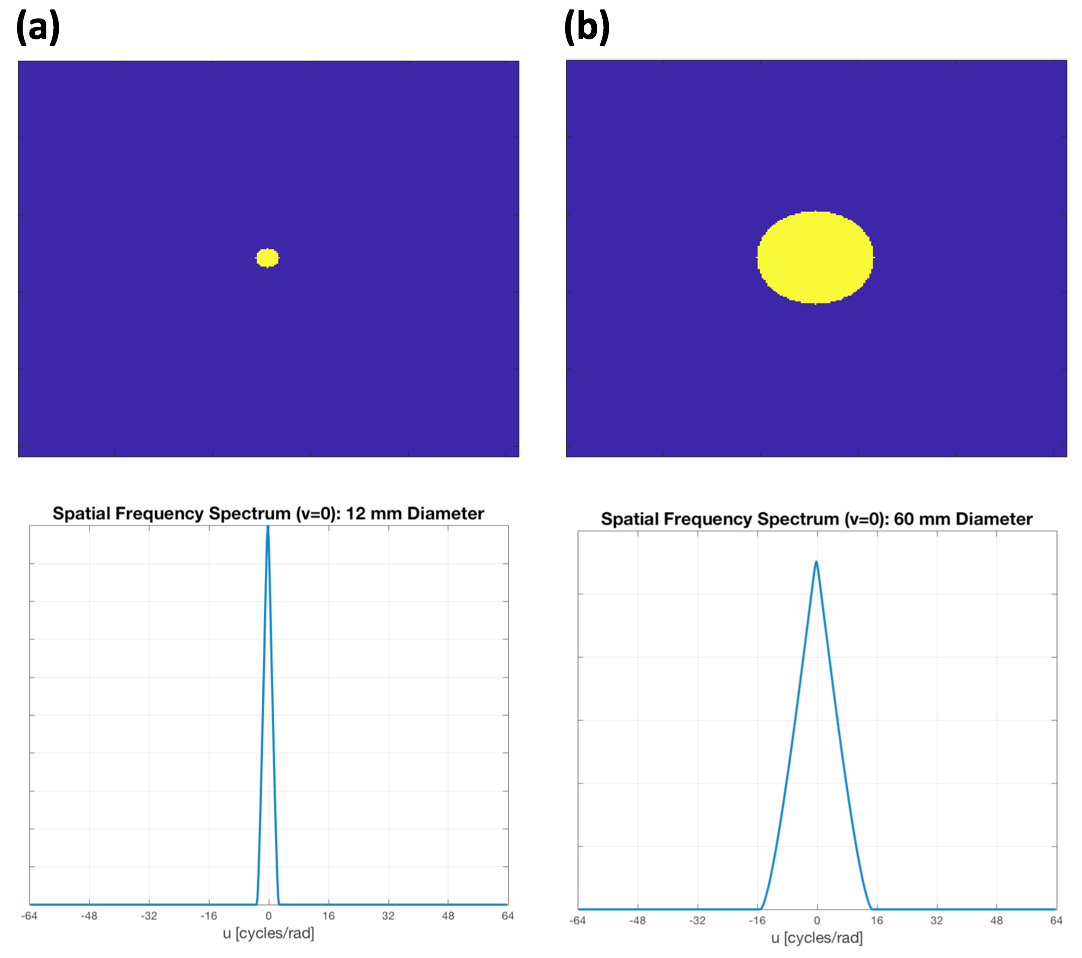
\includegraphics[width=0.45\textwidth]{Figures/VaryDiameter.png}
\caption{Visualization of antenna aperture and the corresponding spatial frequency spectrum or transfer function of the system in the far-field assuming $\lambda$ = 4 mm for (a) a 12 mm diameter aperture and (b) a 60 mm diameter aperture.}
\label{AzResDSize}
\end{figure}
\newline
\indent
To explore potential solutions, we will analyze the spatial frequency spectrum in the far-field. The spatial frequency spectrum is the inverse Fourier Transform of the power pattern or impulse response of the imaging system and therefore can also be referred to as the transfer function of the system in the far-field. Equivalently, the spectrum can also be found via the auto-correlation of the aperture illumination. In order to achieve high azimuth resolution, we ideally want to cover as much of the spatial frequency spectrum as possible. If we had uniform coverage, the power pattern would be a perfect impulse and the imaging system would have ideal azimuth resolution. Referring to the proposed example scenario above, the spatial frequency spectrum can be found in Figure \ref{AzResDSize}(a). It is clear that only the low spatial frequencies would be resolved by this system resulting in poor resolution. One possible solution to covering more of the spectrum is to increase the aperture size. In Figure \ref{AzResDSize}(b), the aperture has been increased by 5 times, and yet the coverage of the spectrum is still poor. It would therefore require an unreasonably large aperture to obtain the desired resolution.
\subsection*{Motivating Synthetic Aperture Radar}
\indent \indent
Another potential solution is the use of two or more apertures. Again, the spatial frequency spectrum can be found via the auto-correlation of the aperture illumination. This has been completed in MATLAB for two, four, and sixteen apertures and is shown in Figure \ref{AzRes}. It is evident that the more apertures in the array, the better the spectral coverage and thus the better the azimuth resolution; however, an array of 16 apertures may be too large, complex, or expensive for system operation. This motivates the use of synthetic aperture radar (SAR). 
\begin{figure}[h!]
    \centering
    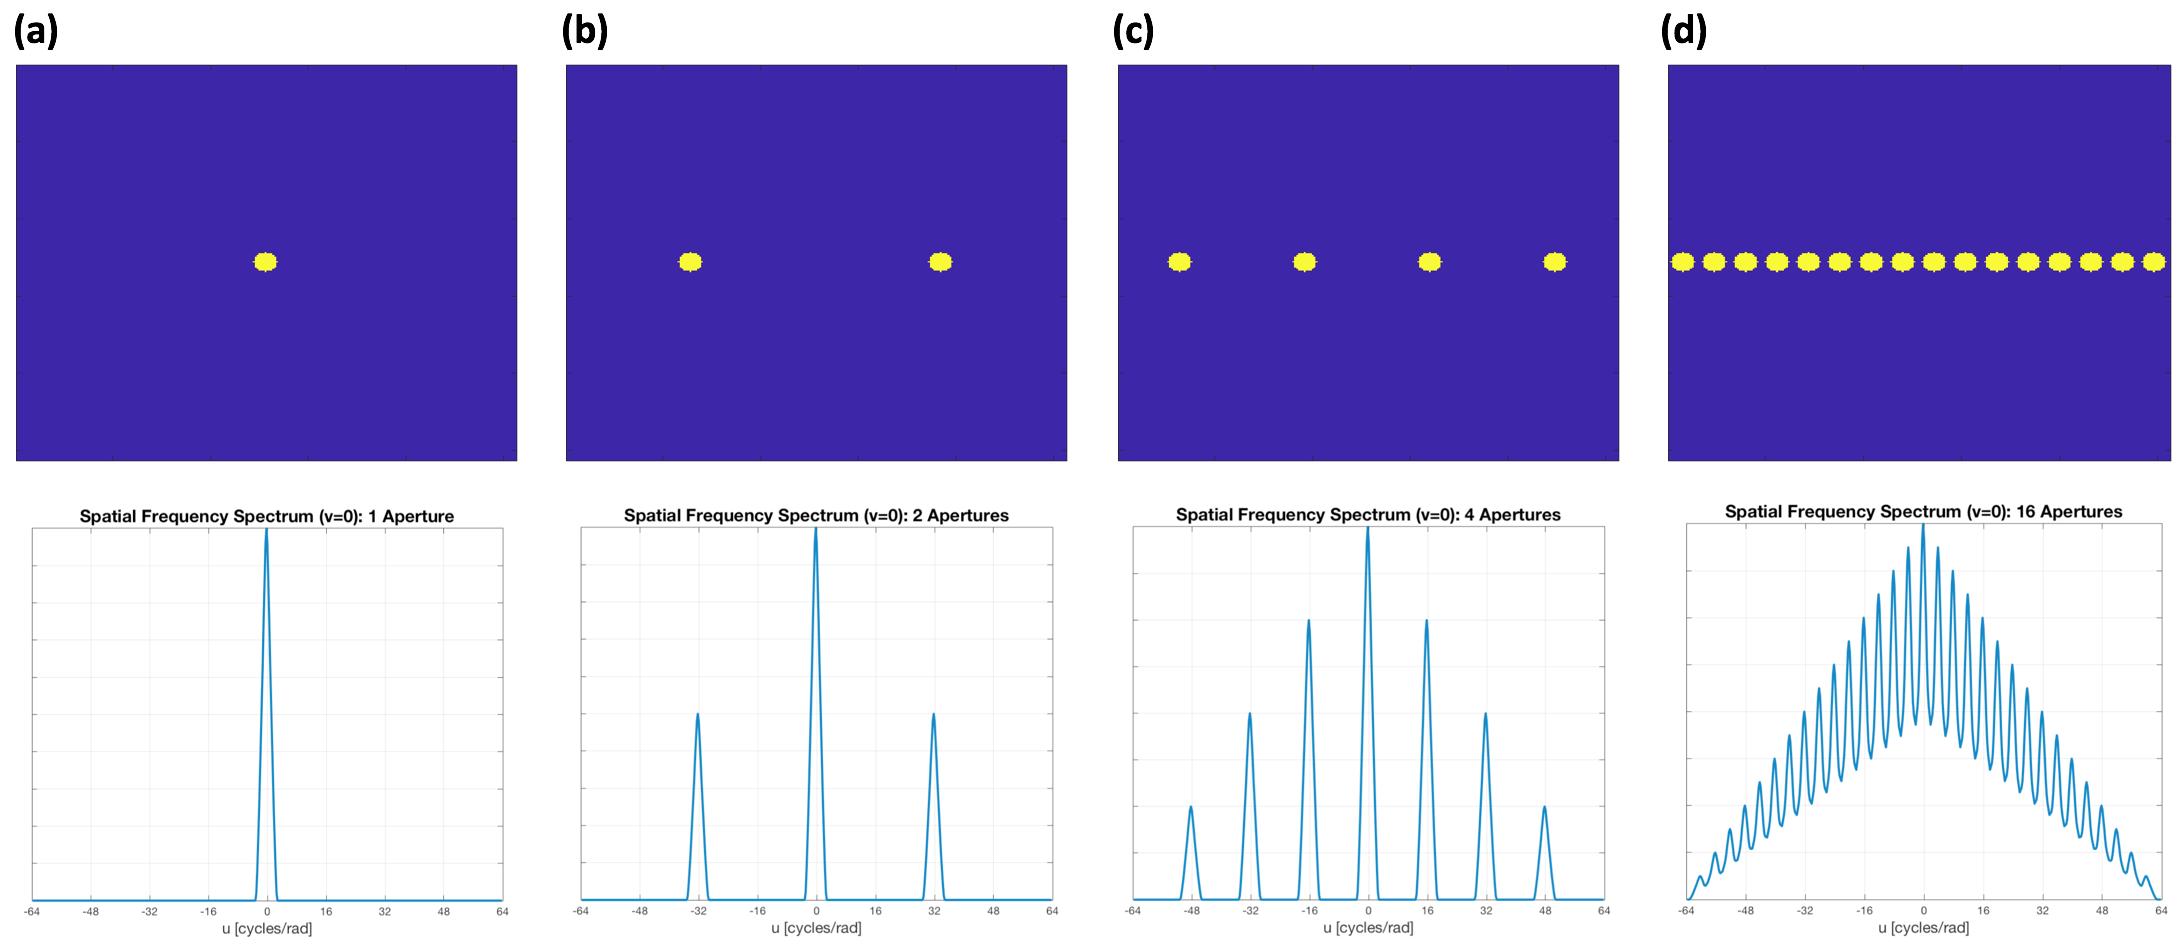
\includegraphics[width=\textwidth]{Figures/AzRes.png}
\caption{Visualization of antenna apertures, each with 12 mm diameter, and the corresponding spatial frequency spectrum or transfer function of the system in the far-field assuming $\lambda$ = 4 mm for (a) 1 aperture, (b) 2 apertures, (c) 4 apertures, and (d) 16 apertures. }
\label{AzRes}
\end{figure}
\newline
\indent
Using synthetic aperture radar, the system can have an array of fewer radar elements or even a single aperture to achieve better resolution through the movement and coherent processing of individual measurements that comprise a large effective aperture. While the degree to which the azimuth resolution can be improved depends on the reconstruction algorithm, the theory presented above holds true. Through the remainder of this paper, we will present two reconstruction algorithms that produce high-resolution images and we will analyze the effect of location errors on image reconstruction.

\section{SAR Background}
\subsection{System Model}
\indent \indent
The goal of SAR is to identify the locations of \( n \) targets, located at coordinates \((x_{n} , y_{n}) \), where \( x \) is the range domain and \( y \) is the cross-range
    (or azimuth) domain. Our radar is located at \((0,u) \) and emits a large-bandwidth signal \( p(t) \). The radar radiation pattern is assumed to be uniform for now. The receiver is colocated with the transmitter, and receives the following signal:
\begin{displaymath}
    s(t,u) = \sum\limits_{n}^{} \sigma_{n} p \left[ t - \frac{2 \sqrt{x_{n}^2 +(y_{n} - u)^2}}{c}  \right]
\end{displaymath}
The time delay \( \frac{2 \sqrt{x_{n}^2 +(y_{n} - u)^2}}{c} \) is the round-trip delay from the transmitter/receiver to the nth target. The \( \sigma_{n} \) term incorporates both the radar reflectivity of our target (which is assumed to be frequency independent here, although in general this is not the case), as well as the amplitude function \( \frac{1}{\sqrt{x_{n}^2 + y_{n}^2}} \), which results from the inverse-square power law for propagating waves. We sweep the radar over an aperture range \((0,u) \) to record the echoed signal \( s(t,u) \).
\begin{figure} [h!]
    \centering
    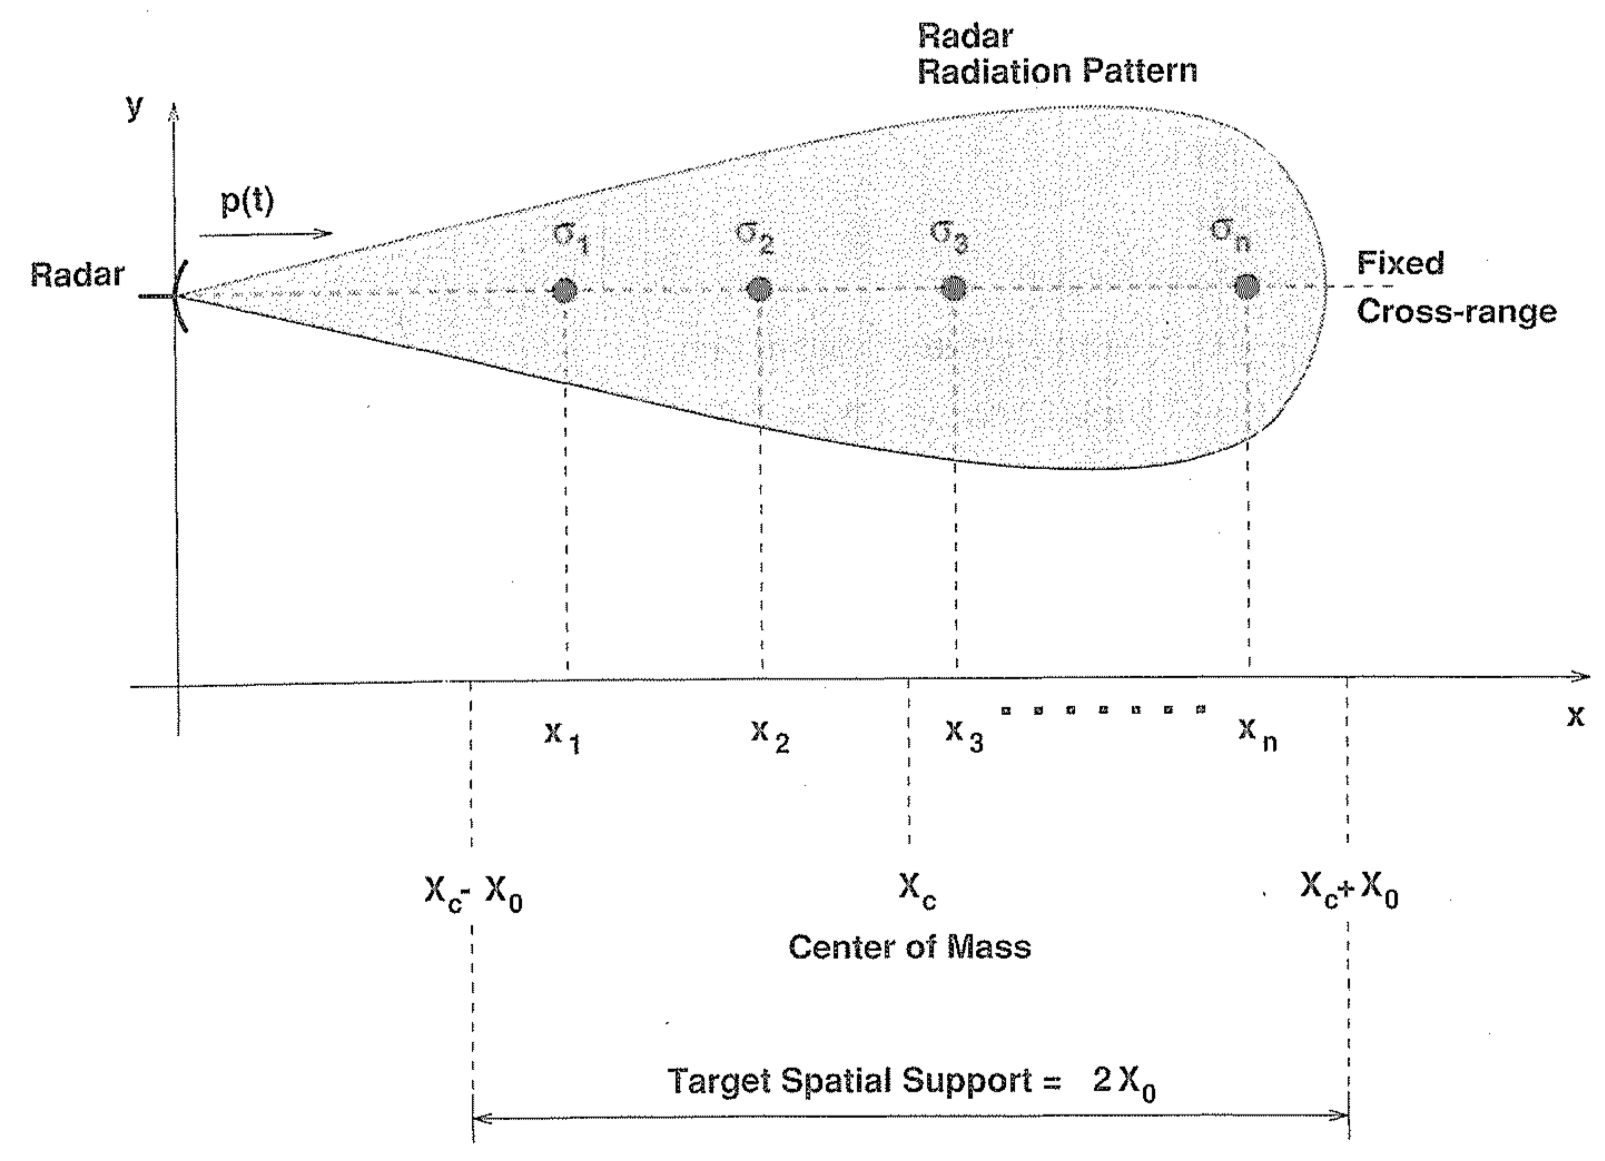
\includegraphics[width=0.5\textwidth]{Figures/range_diagram.png}
    \caption{1D Radar Range Imaging}
    \label{range_diagram}
\end{figure}


\section{Traditional SAR Reconstruction Algorithms}
\subsection{Range-Doppler Reconstruction}
We begin by describing the Range-Doppler Reconstruction algorithm because it was one of the earliest SAR algorithms to be widely implemented, it is only an approximate solution, and it directly builds off of the material covered in EE262. While we did not implement the Range-Doppler algorithm in MATLAB, we believe that its explanation helps motivate the interest in alternative algorithms. As we shall soon demonstrate, the Range-Doppler algorithm is based on Fresnel approximation and thus assumes a narrow beam width and treats reconstruction as a separable two-dimensional problem, which as we demonstrated above is not true. We begin with the fast-time Fourier transform of our radar signal:
\begin{displaymath}
	s( \omega , u) = P(\omega) \sum\limits_{n}^{} \sigma_{n} exp\left[ -2jk \sqrt{(X_{c} + x_{n})^2 +(y_{n} - u)^2} \right] 
\end{displaymath}
We can take the Taylor Series expansion of the exponential term, which represents the round-trip distance from the nth target to the radar, around \( X_{c} \):
\begin{displaymath}
	\sqrt{(X_{c} + x_{n})^2 +(y_{n} - u)^2} = X_{c} + x_{n} + \frac{(y_{n} - u) sq}{2 X_{c} } + ...
\end{displaymath}
If we neglect the higher order terms, we arrive at
\begin{align*}
	s( \omega , u) &\approx P(\omega) \sum\limits_{n}^{} \sigma_{n} exp\left[ -2jk(X_{c} + x_{n}) - j k \frac{(y_{n} - u)^2 }{X_{c}} \right]\\
				   &= P(\omega) exp(-2jk X_{c} ) \sum\limits_{n}^{} \sigma_{n} exp\left[ -2jk x_{n} - j \frac{k(y_{n} - u)^2}{X_{c}} \right], 
\end{align*}
which we recognize as the Fresnel approximation for the SAR signal. Now we consider the ideal target function and its spatial fourier transform with respect to the range domain, defined as follows
\begin{align*}
	f_0(x,y) &= \sum\limits_{n}^{} \sigma_{n} \delta(x - x_{n} , y - y_{n}) \\
	F_{0x}(k_{x} , y) &= \sum\limits_{n}^{} \sigma_{n} exp(-j k_{x} x_{n}) \delta (y - y_{n}) 
\end{align*}
Now we can rewrite the Fresnel approximation as
\begin{displaymath}
	s(\omega , u) \approx P(\omega) F_{0x}(2k , y) * exp\left( -j \frac{k u^2}{X_{c} }\right)
\end{displaymath}
where * is convolution in the slow-time domain. To recover the target function \( f(x,y) \), we can use a matched filter to removed the exponential function:
\begin{displaymath}
	F_{x}(k_{x} , y) \approx P(\omega)^{*} s(\omega , u) *exp\left(j \frac{k u^2 }{X_{c} }\right)
\end{displaymath}
If we make the assumption that the radar bandwidth is much smaller than the carrier frequency, then we can approximate \( k \approx k_{c} \). This allows us to perform the above matched filter operation separately along the fast-time and slow-time domains:
\begin{align*}
	F_{x}(k_{x} , y) &\approx P(\omega)^{*} s(\omega, u) * exp\left(j \frac{k_c u^2 }{X_{c} }\right)\\
	k_{x} &= 2k = \frac{2 \omega}{c} \\
	y &= u
\end{align*}
Therefore we obtain
\begin{align*}
	f(x,y) &\approx s(t,u) * p(-t)^{*} * exp\left(j \frac{k_c u^2 }{X_{c} }\right)\\
		   &= s_{M}(t,u) * exp\left(j \frac{k_c u^2 }{X_{c} }\right)
\end{align*}






\subsection{Backprojection}
\indent\indent
Backprojection is a commonly used algorithm in SAR imaging that results in high resolution reconstructed images in both the range and azimuth directions. The driving principle of backprojection is tracing back the received signal in the time domain to the location of the corresponding reflector. With a single receive aperture, the direction from which the signal arrives, or the reflector location in azimuth, is unknown; however, using SAR imaging, this limitation can be overcome. In this section, we will explain the theory of the backprojection algorithm in SAR imaging and produce complementary simulation results.
\newline
\indent
Backprojection achieves high range-resolution through the matched filtering technique explained in Section 2. The first step of the algorithm is to obtain the matched filtered SAR signal by correlating the received SAR signal with the transmitted pulse, typically a chirp.
\begin{equation}
\label{mf_sig}
s_M(t,u) = s(t,u) \ast p_0^{\ast}(-t),
\end{equation}
where $p_0(t)$ is the transmitted pulse, $t$ is the time, and $u$ is the aperture location in the direction of radar movement, often referred to as fast-time and slow-time, respectively, in SAR \cite{SARbook}. The matched filtered SAR signal has peaks at times that correspond to the time of arrival of the echos from targets within the scene. For example, if the target in the scene is at position $(x_1,y_1)$, then $s_M(t,u)$ will have a peak at time:
\begin{equation}
\label{tof_example}
t = \frac{2\sqrt{x_1^2+(y_1-u)^2}}{c},
\end{equation}
where $c$ is the speed of light and the factor of two is a result of two-way travel to and from the radar. 
\newline
\indent
Now, if we create an array for the reconstructed image, $im(x_i,y_i)$, we can begin assigning the matched filtered SAR signal to the proper pixels for each aperture location. Note that care must be taken to upsample the matched filtered SAR signal to reverse the demodulation that occurs in the radar front-end hardware before performing some of these computations; however, we neglect it here for simplicity. In order to assign the pixel values properly, we must first know the time of arrival for each pixel in $im(x_i,y_i)$ that represents our scene. This can be computed similarly to \eqref{tof_example}, but rather now as an array of time values:
\begin{equation}
\label{tof_array}
t_{ij}(u) = \frac{2\sqrt{x_i^2+(y_j-u)^2}}{c}.
\end{equation}
\newline
\indent
Refer to Figure \ref{SceneMap} for a diagram that explains this mapping. For each pixel in $im(x_i,y_i)$, there is an associated time, $t_{ij}$. At each aperture location, a SAR signal is received and the matched filtered signal is computed. The image pixels can then be looped through assigning the sampled matched filtered signal value at the time corresponding to $t_{ij}$ to the reconstructed image, $im(x_i,y_j)$. The process of computing a time of arrival array and matched filtered SAR signal must be repeated at each aperture location due to their dependence on the aperture location, $u$. The image can be represented by the equation:
\begin{equation}
\label{IM}
im(x_i,j_i) = \sum_{u}s_M(t_{ij}(u),u).
\end{equation}
\begin{figure}[h!]
    \centering
    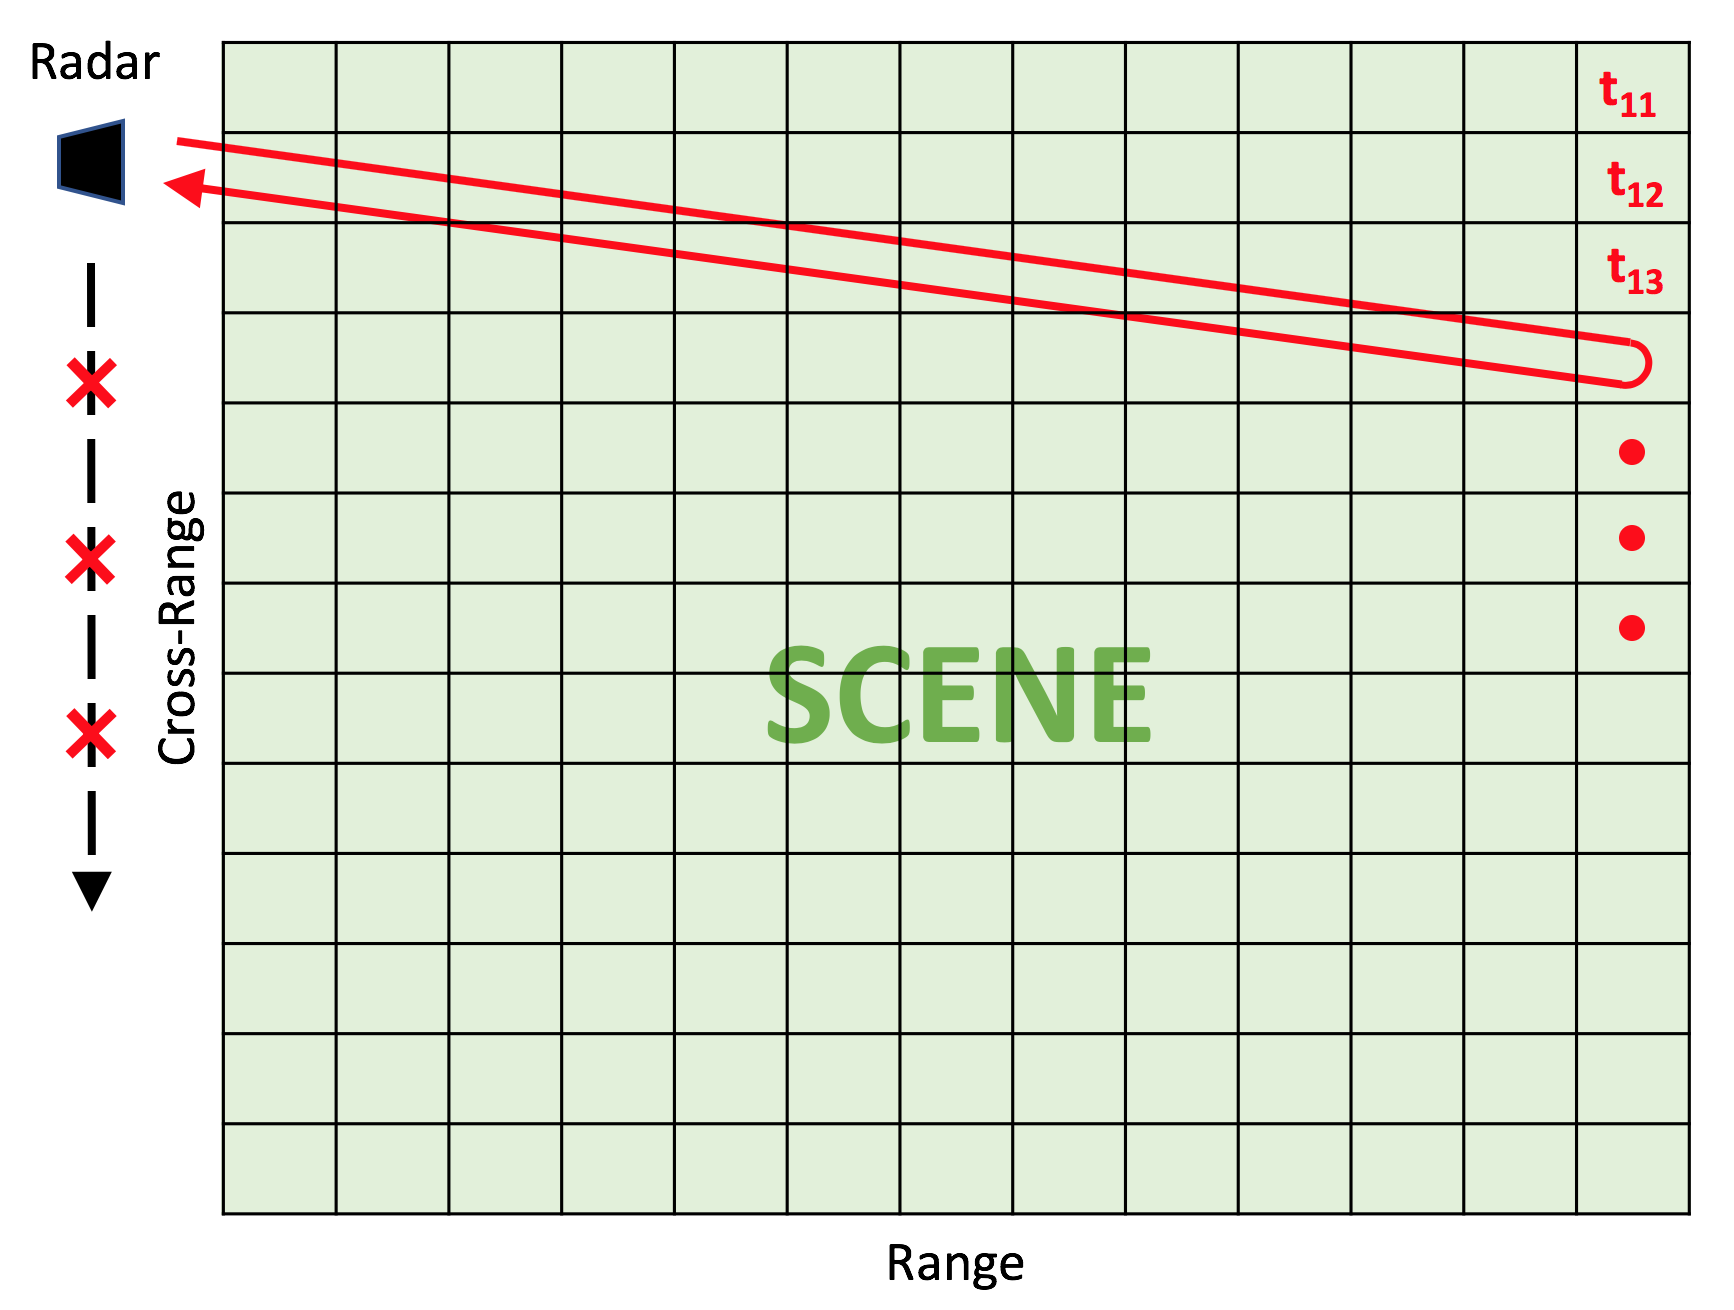
\includegraphics[width=0.4\textwidth]{Figures/SceneMap.png}
\caption{Mapping of the time array to the image pixels that is later used for assigning signal values to the image pixels. The aperture does not move during creation of the time array. This mapping must be done for each aperture location.}
\label{SceneMap}
\end{figure}
\newline
\indent
For a single aperture location, there will be many pixels that have the same time of arrival. This will result in an arc through each target in the reconstructed image as depicted in Figure \ref{BPRecons}(a). As we increase the number of apertures, the arcs will intersect only at the location of the targets in the scene as seen in Figure \ref{BPRecons}(b). There are fewer arcs than there are aperture locations as a result of scans for which the target fell out of the radar beam-width as well as some scans that fell into the same time bins. If we scan our aperture across the entire scene of interest with a half-wavelength spacing (typical in practical application for no grating lobes or over-sampling), then we achieve the high resolution image in Figure \ref{BPRecons}(c). There are no arcs visible in this image due to the target location having significantly higher intensity than surrounding pixels. The parameters used in the MATLAB simulation to produce these example reconstructed images can be found in Table \ref{table:1}.
\begin{figure}[h!]
    \centering
    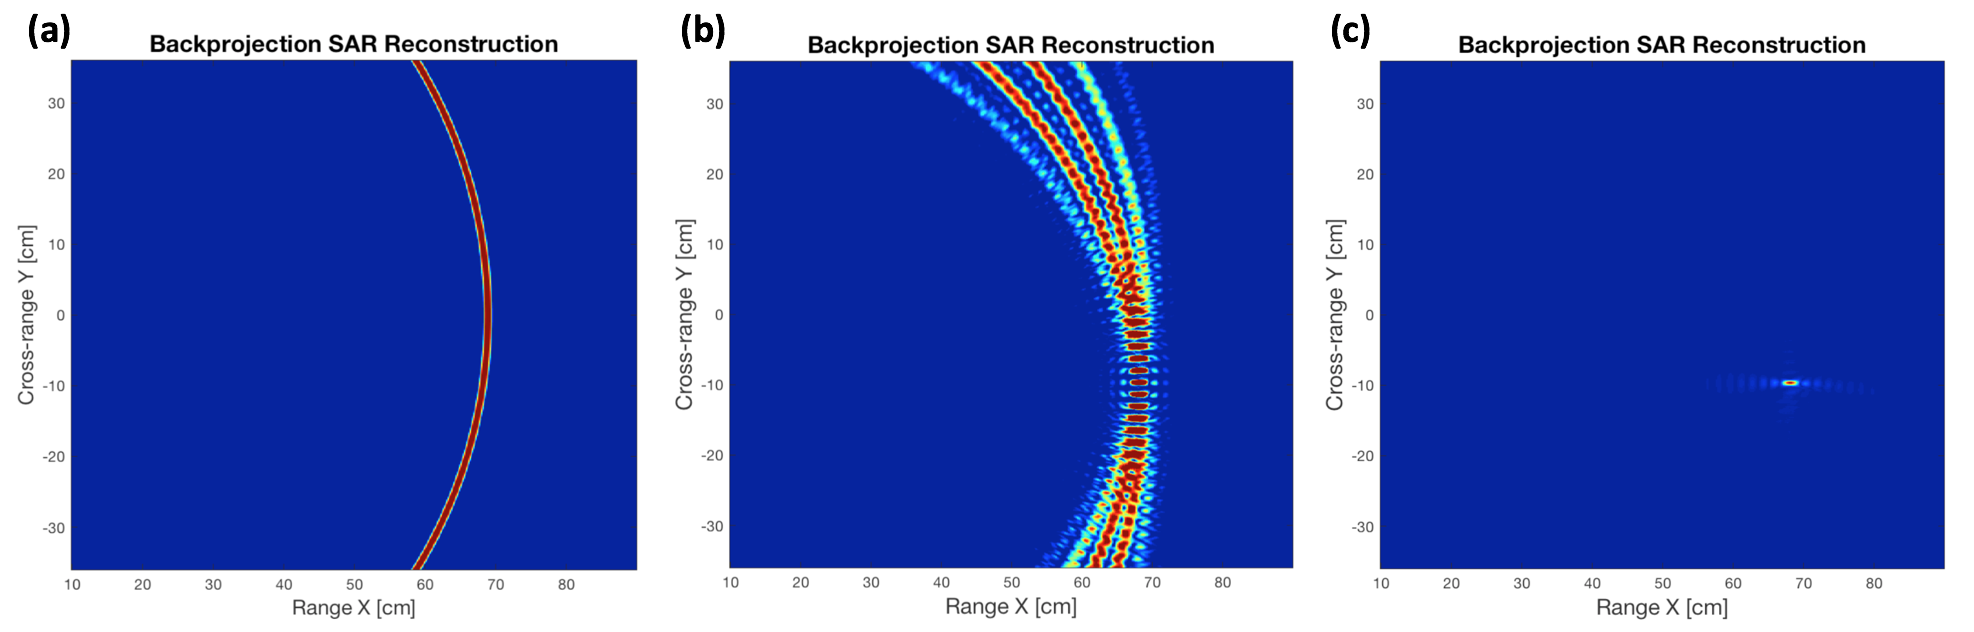
\includegraphics[width=\textwidth]{Figures/BackprojectionRecons.png}
\caption{Reconstructed images of one target in a scene using backprojection for (a) a single aperture measurement at (0,0), (b) 18 scans spanning the full scene with aperture locations spaced by $20{\lambda}$, and (c) full scene scan with aperture locations spaced by $\frac{\lambda}{2}$}
\label{BPRecons}
\end{figure}
\begin{table}[h!]
\begin{center}
\begin{tabular}{ |c|c| } 
 \hline
 \textbf{Simulation Parameter} & \textbf{Value} \\ 
 \hline
 Carrier Frequency & 77 GHz \\ 
 \hline
 Chirp Bandwidth & 5 GHz \\ 
 \hline
 Chirp Duration & 17 ns \\ 
 \hline
 Aperture Diameter & 8.3 mm \\ 
 \hline
 Synthetic Aperture Length & 1.3 m \\ 
 \hline
\end{tabular}
\caption{Parameters used for MATLAB simulations.}
\label{table:1}
\end{center}
\end{table}

\subsection{2D Matched Filtering and Interpolation}
\subsubsection*{2D Matched Filtering}
We begin 2D the Matched Filtering and Interpolation reconstruction by taking the fast-time Fourier transform of the received signal \( s(t,u) \):
\begin{displaymath}
	s( \omega , u) = P( \omega) \sum\limits_{n}^{} \sigma_{n} exp\left[ -2jk \sqrt{x_{n}^2 +(y_{n} - u)^2} \right]
\end{displaymath}
where \( k = \omega / c \) is the wavenumber. We then take the slow-time Fourier transform of \( s( \omega , u) \):
\begin{displaymath}
	S( \omega , k_{u}) = P(\omega) \sum\limits_{n}^{} \sigma_{n}exp(-j \sqrt{4 k^2 - k_{u}^2} x_{n} - j k_{u} y_{n} ) 
\end{displaymath}
We can rewrite the above expression by defining the following SAR spatial frequency transformation functions:
\begin{align*}
	k_{x}(\omega , k_{u}) &= \sqrt{4 k^2 - k_{u}^2} \\
	k_{y}(\omega , k_{u}) &= k_{u}
\end{align*}
Substituting:
\begin{displaymath}
	S( \omega , k_{u}) = P(\omega) \sum\limits_{n}^{} \sigma_{n}exp[-j k_{x}(\omega , k_{u} ) x_{n} - j k_{y}(\omega , k_{u}) y_{n} ]
\end{displaymath}
We also introduce the ideal target function and its Fourier transform:
\begin{align*}
	f_0(x,y) &= \sum\limits_{n}^{} \sigma_{n} \delta(x - x_{n} , y - y_{n}) \\
	F_0(k_{x} , k_{y}) &= \sum\limits_{n}^{} \sigma_{n} exp(-j k_{x} x_{n} - j k_{y} y_{n}) 
\end{align*}
We observe that \( S(\omega , k_{u}) \) and \( F_0(k_{x} , k_{y}) \) are both linear phase functions of \((x_{n}, y_{n} )  \). Substituting the above expression for \( F_0(k_{x} , k_{y}) \) into \( S(\omega , k_{u}) \), we get
\begin{align*}
	S(\omega , k_{u}) &= P(\omega) F_0 [k_{x}(\omega , k_{u}) , k_{y}(\omega , k_{u}) ] \\
	F_0 [k_{x}(\omega , k_{u}) , k_{y}(\omega , k_{u}) ] &= \frac{S(\omega , k_{u})}{P(\omega)}\\
\end{align*}
We can not perform the above operation because neither \( S \) nor \( P \) are nonzero over all \( \omega \). Instead, we perform fast-time matched filtering:
\begin{align*}
	F [k_{x}(\omega , k_{u}) , k_{y}(\omega , k_{u}) ] &= P^{*}(\omega) S(\omega , k_{u}) \\
														 &= |P^{*}(\omega)|^2 \sum\limits_{n}^{} \sigma_{n} exp(-j k_{x} x_{n} - j k_{y} y_{n})
\end{align*}
\subsubsection*{Interpolation}
Thus far, we have arrived at an expression for \( F(k_{x} , k_{y}) \), from which we can take the 2D inverse Fourier transform and obtain \( f(x,y) \). However, the spatial frequency variables \( (k_{x}, k_{y}) \) are defined in terms of a nonlinear mapping of \((\omega , k_{u}) \). We collect an evenly spaced grid of points in the \((\omega , k_{u}) \) domain, but after the nonlinear mapping we have a non-evenly spaced grid of \( (k_{x}, k_{y}) \).
This sampling relationship is demonstrated in Figure \ref{SAR_spatial_freq_map}. Therefore, we need to interpolate a uniform grid of \( (k_{x}, k_{y}) \) points from the grid of \((\omega , k_{u}) \) points.

If we have \( M \) synthetic aperture samples, each with a spacing \( \Delta_{u} \) in the \( u \)domain, we will have \( M \) samples in the \( k_{u} \) domain with the following spacing:
\begin{displaymath}
	\Delta_{k_{u}} = \frac{2 \pi}{M \Delta_{u}} 	
\end{displaymath}
We also notice that \( k_{y} = k_{u} \), which means we have samples of \( S(\omega , k_{u}) \) at evenly spaced values of \( k_{u} \). However, this is not the case for
\begin{displaymath}
	k_{x}(\omega , k_{u}) = \sqrt{4 k^2 - k_{u}^2}
\end{displaymath}
We define \( k_{ymn} \) as the available cross-range spatial frequency sampled points, \( k_{um} \) as the slow-time Doppler samples points for the SAR signal. We obtain the relation
\begin{displaymath}
	k_{ymn} = k_{um} = m \Delta_{k_{u}}
\end{displaymath}
We want to obtain equally spaced values for \( k_{xmn} \), which we define as the available range spatial frequency sampled points:
\begin{displaymath}
	k_{xmn} = \sqrt{4 k_{n}^2 - k_{um}^2} 
\end{displaymath}
where
\begin{displaymath}
	k_{n} = n \Delta_{k} = n \frac{\Delta_{w}}{c} 
\end{displaymath}
If we assume that we are interpolating from evenly spaced data, i.e. \( k_{xn} = n \Delta_{k_{x}} \), we can use the following interpolation equation:
\begin{displaymath}
	F(k_{x} , k_{ymn}) = \sum\limits_{n}^{} F(n \Delta_{k_{x}} , k_{ymn}) h(k_{x} - n \Delta_{k_{x}}) 
\end{displaymath}
where the interpolating function is defined as
\begin{displaymath}
	h(k_{x}) = sinc \left( \frac{k}{\Delta_{k_{x}}} \right)
\end{displaymath}
This concludes the 2D Matched Filter and Interpolation reconstruction algorithm.

\begin{figure}[h!]
    \centering
    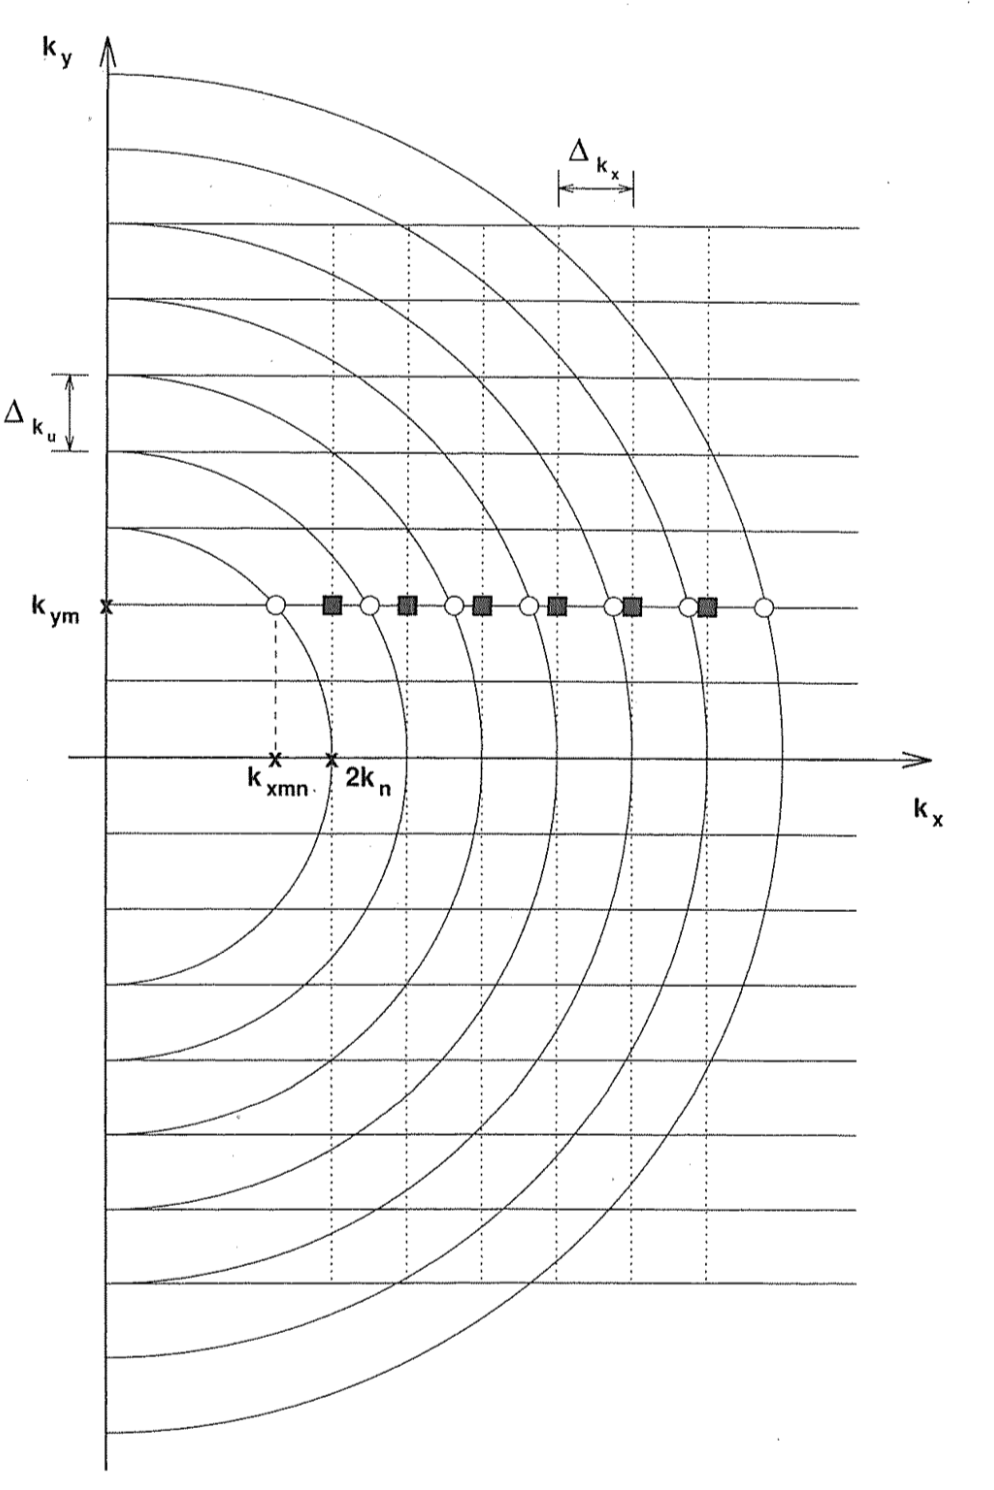
\includegraphics[width = .5\textwidth]{Figures/SAR_spatial_freq_map.png}
    \caption{SAR Spatial Frequency Mapping}
    \label{SAR_spatial_freq_map}
\end{figure}

\section{Theoretical and Simulated Effects of Location Errors}
\indent\indent
In synthetic aperture radar systems, one practical issue is the effect of aperture location errors as a result of variable speeds of the radar-carrying vehicle. Due to the fact that the reconstruction algorithms rely on knowledge of the aperture location for each acquired measurement, a global positioning system (GPS) is often placed on the radar carrying vehicle providing at best centimeter accuracy \cite{SARbook}. 
\newline
\indent
As we have mentioned previously, a typical aperture spacing is a half-wavelength to avoid grating lobes and over-sampling. When operating at lower frequencies, aperture location errors on the order of centimeters are negligible due to the relatively long wavelengths. However, a millimeter wave radar system operating at a center frequency of, for example 77 GHz, has a wavelength of less than 4 millimeters, rendering GPS with centimeter accuracy practically useless. In this section, we explore the effect of aperture location errors on image reconstruction for the 2D matched filtering and interpolation algorithm as well as for the backprojection algorithm and propose the use of a neural network to compensate for these errors and reconstruct high-quality images.
\subsection{2D Matched Filtering and Interpolation}
We introduce location error $\epsilon$ into the cross-range location $u$ of the sensor: \( s(t,u + \epsilon) \). Since our error is assumed to be Gaussian with mean $\mu$ and variance $\sigma^2$, the Fourier transform of $\epsilon$ is $\mathcal{E}$, which is also a Gaussian distribution. We omit scaling for simplicity. We can trace this error through the reconstruction equations beginning with:
\begin{displaymath}
	s( \omega , u + \epsilon) = P( \omega) \sum\limits_{n}^{} \sigma_{n} exp\left[ -2jk \sqrt{x_{n}^2 +(y_{n} - (u + \epsilon)^2} \right]
\end{displaymath}
\begin{displaymath}
	S( \omega , k_{u} + \mathcal{E}) = P(\omega) \sum\limits_{n}^{} \sigma_{n}exp(-j \sqrt{4 k^2 - (k_{u} + \mathcal{E})^2} x_{n} - j (k_{u}+\mathcal{E}) y_{n} ) 
\end{displaymath}
\begin{align*}
	k_{x}(\omega , k_{u} + \mathcal{E}) &= \sqrt{4 k^2 - (k_{u}+\mathcal{E})^2} \\
	k_{y}(\omega , k_{u}+ \mathcal{E}) &= k_{u} + \mathcal{E}
\end{align*}
We can trace this through to:
\begin{align*}
	k_{x} &= \sqrt{4 k^2 - (k_{u} + \mathcal{E})^2} \\
	F(k_{x} , k_{ymn}) &= \sum\limits_{n}^{} F(n \Delta_{k_{x}} , m \Delta_{k_{u}+\mathcal{E}}) h(k_{x} - n \Delta_{k_{x}}) \\
\end{align*}
The above equations give the Fourier transform of our target function $f(x,y)$ as a function of the Fourier transform of the error $\epsilon$. Since the interpolation function is a function of $k_u$, we see that an error in cross-range position creates error in both the range and cross-range reconstruction, which is supported by the plots showing Gaussian location error for several levels of noise (see Figures \ref{2dvar0} - \ref{2dvar4}).

\begin{figure}[h!]
    \centering
    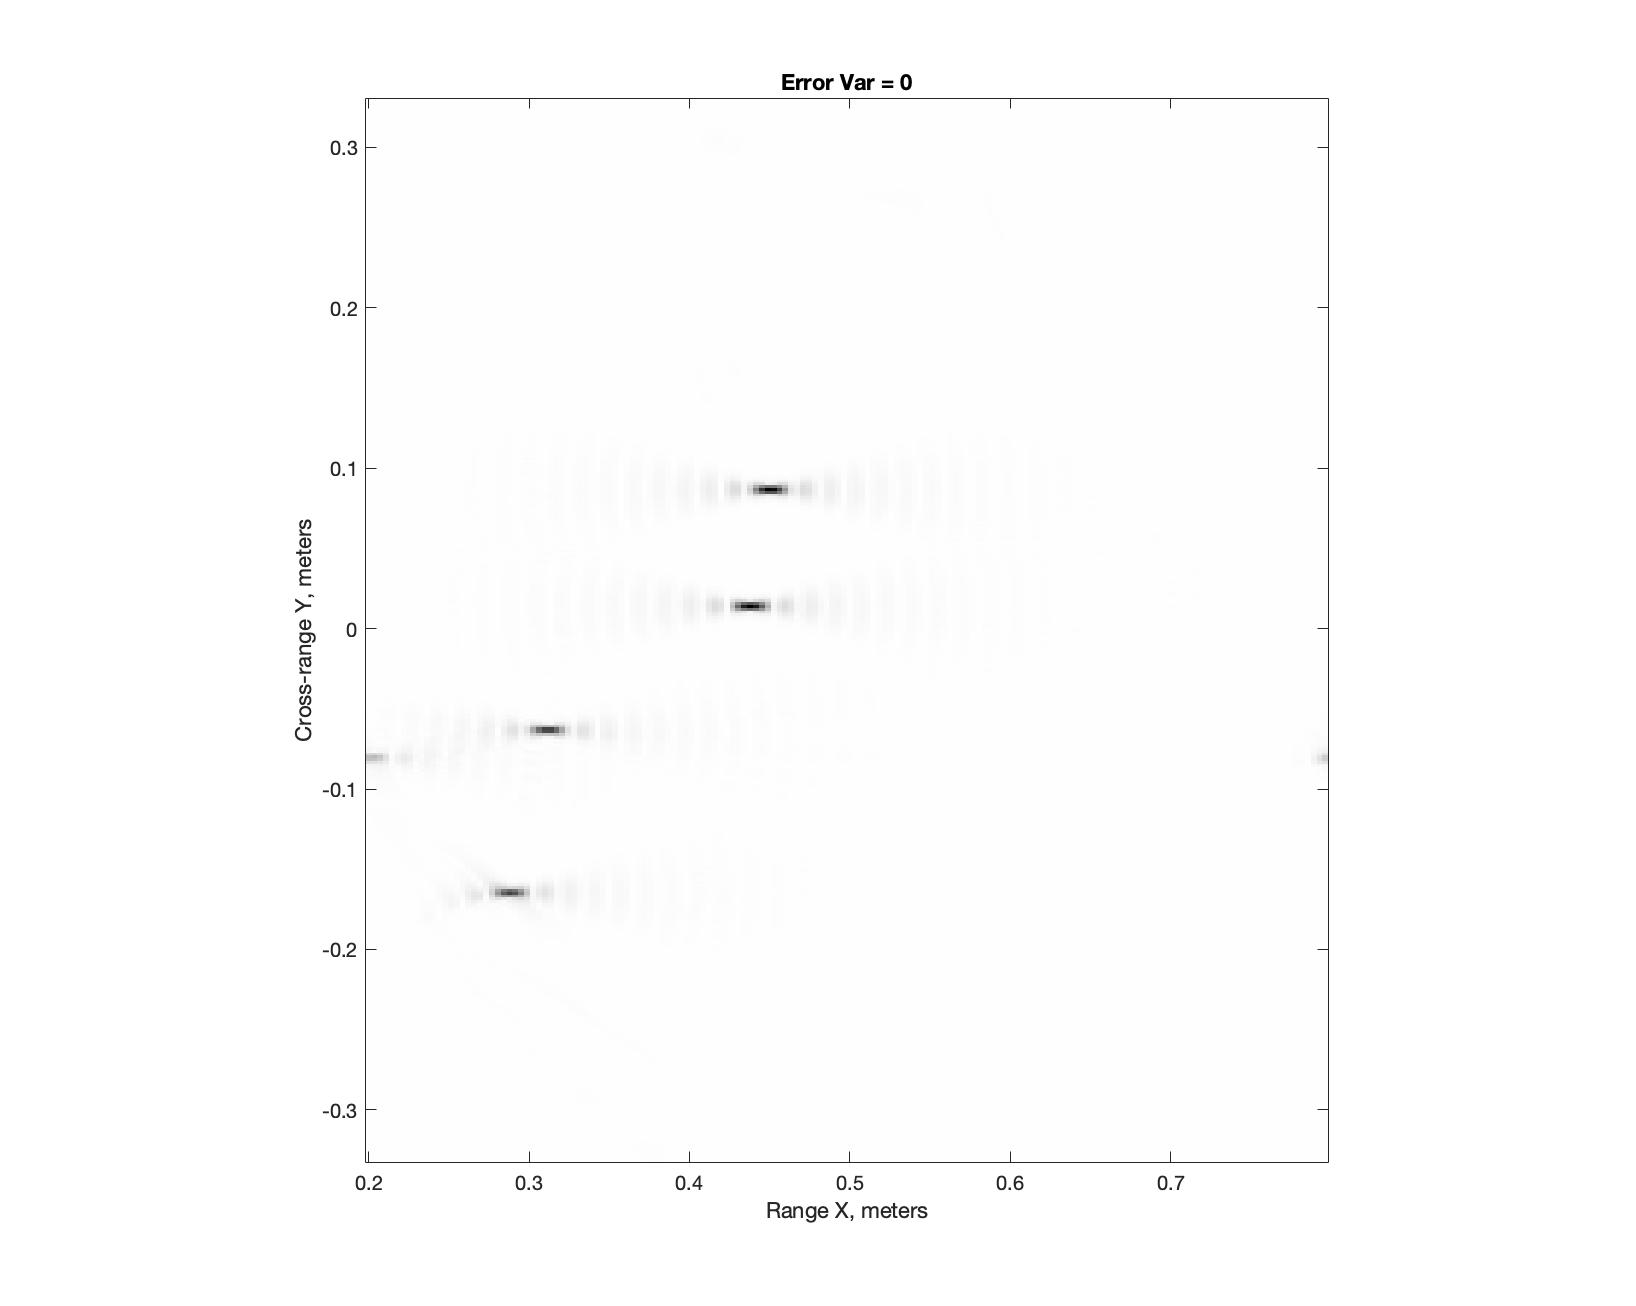
\includegraphics[width=.6\textwidth]{Figures/2dvar0.jpg}
    \caption{2D Interpolation \& Reconstruction: No Location Error}
        \label{2dvar0}
\end{figure}
\begin{figure}[h!]
    \centering
    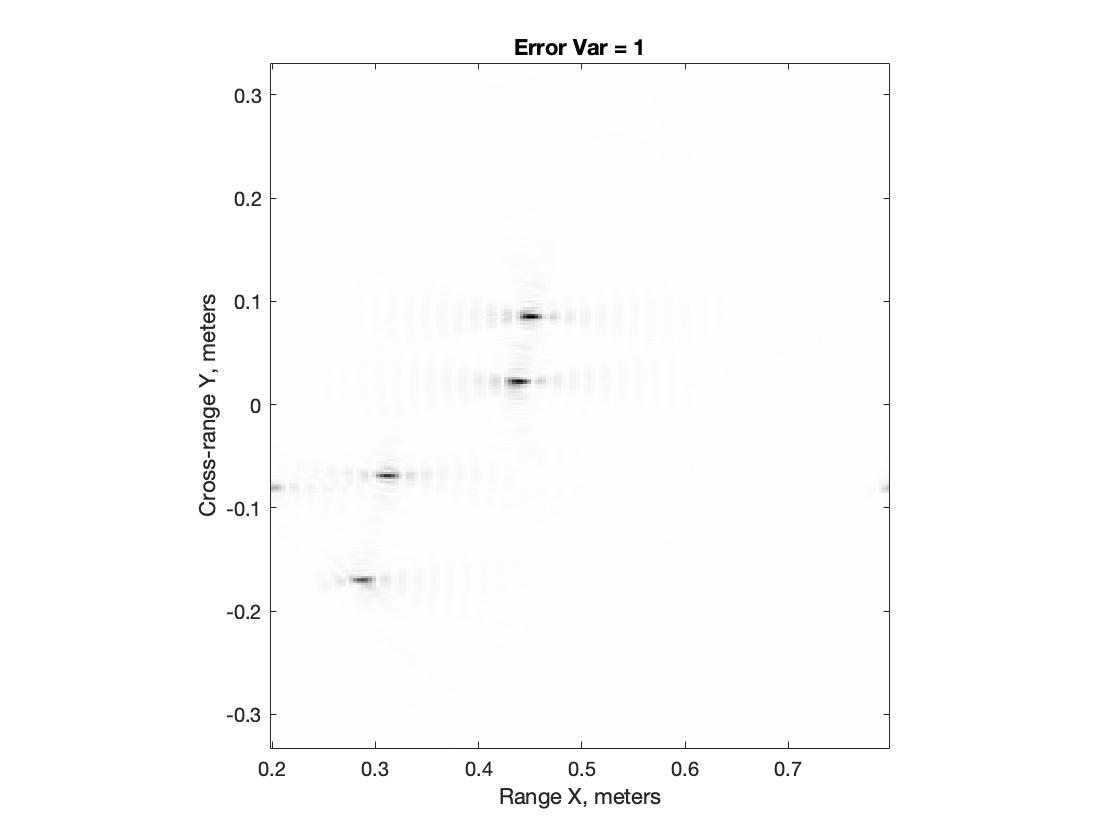
\includegraphics[width=.6\linewidth]{Figures/2dvar1.jpg}
    \caption{2D Interpolation \& Reconstruction: Error $\sigma=\frac{\lambda}{8}$ (500 $\mu${m})}
    \label{2dvar1}
\end{figure}
\begin{figure}[h!]
    \centering
    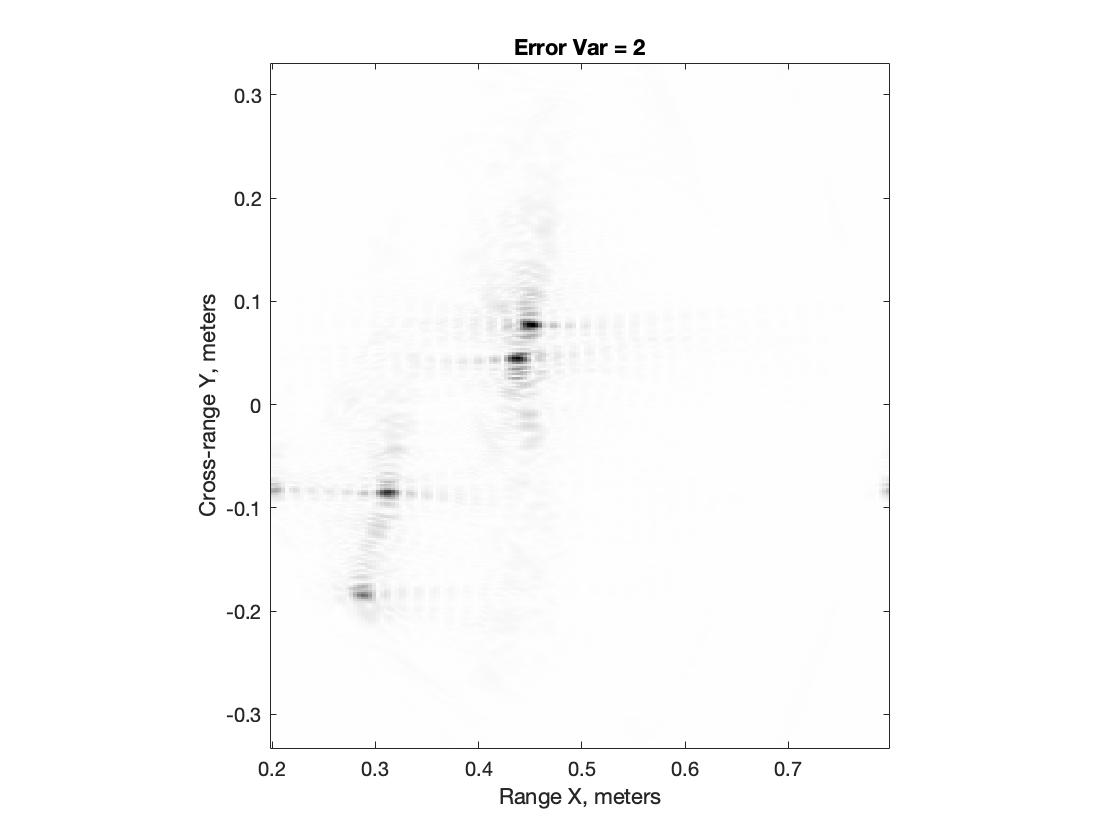
\includegraphics[width=.6\linewidth]{Figures/2dvar2.jpg}
    \caption{2D Interpolation \& Reconstruction: Error $\sigma=\frac{\lambda}{4}$ (1 mm)}
    \label{2dvar2}
\end{figure}
\begin{figure}[h!]
    \centering
    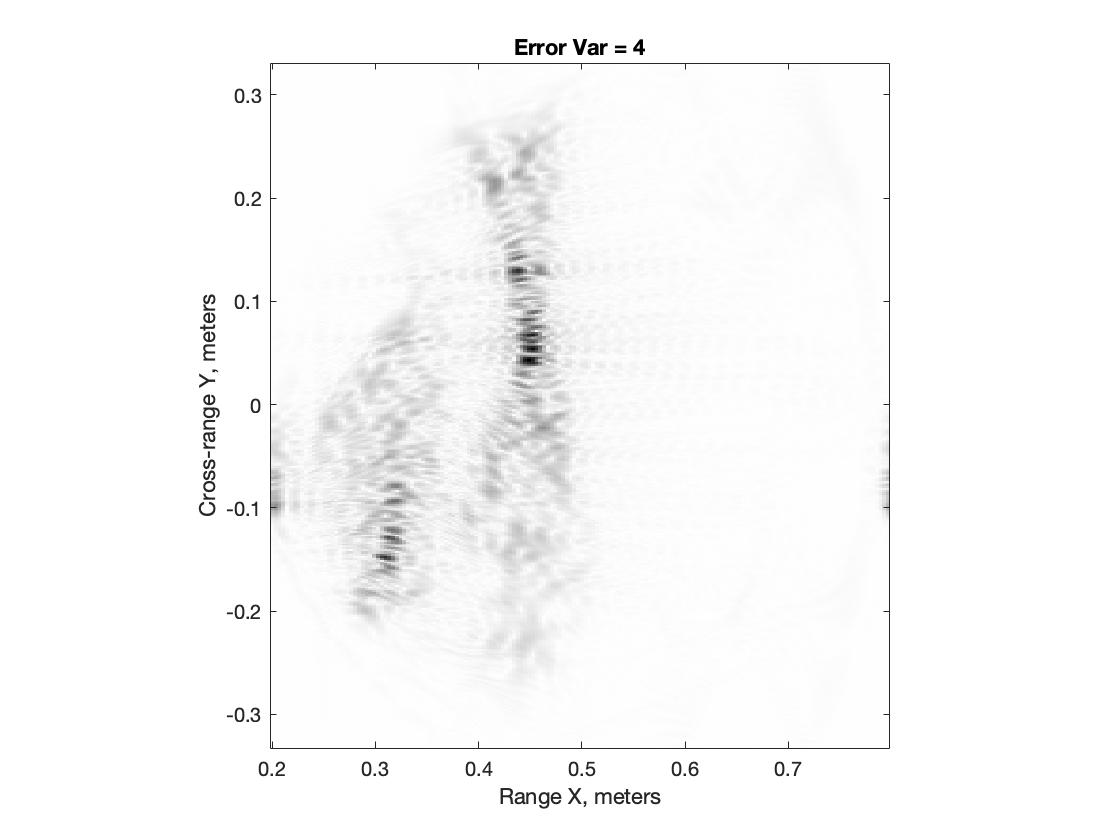
\includegraphics[width=.6\linewidth]{Figures/2dvar4.jpg}
    \caption{2D Interpolation \& Reconstruction: Error $\sigma=\frac{\lambda}{2}$ (2 mm)}
    \label{2dvar4}
\end{figure}


\subsection{Backprojection}
\indent \indent
To begin our analysis of location errors in a practical SAR system, we first must determine the proper modelling. A SAR system operates by transmitting pulses at a given pulse repetition frequency for which echoes from a single pulse characterize a single measurement. The pulse repetition frequency (PRF) is determined by relating the desired aperture spacing to the designed velocity of the radar carrying vehicle. The pulse repetition frequency is fixed, while the velocity of the vehicle may change, resulting in location errors. With this in mind, we note that the proper modelling of the aperture location has cumulative error as follows:
\begin{equation}
\label{Ap_location}
u'(a) = u_0+\sum_{n=1}^{a}\frac{n\lambda}{2}+N(0,n) = u(a)+\sum_{n=1}^{a}N(0,n),
\end{equation}
where $u_0$ is the starting location of the aperture, and $u'(a)$ is the location for the $a^{th}$ movement of the aperture. Since, the error in location is cumulative as a result of the fixed PRF and each error is modelled as normally distributed and assumed independent for simplicity, the variances of the errors add directly, hence $N(0,n)$. 
\newline
\indent
Using our model for location errors of the aperture, we can now analyze how the error propagates through the backprojection reconstruction algorithm. The critical dependencies on the aperture location in the backprojection algorithm are in the creation of the time of arrival array and on the matched filtered SAR signal. Firstly, it is clear that the received SAR signal will be affected by the aperture location error and thus the matched filtered version of the signal will as well. The matched filtered SAR signal will have a phase error that corresponds to the location error as derived below and as illustrated in Figure \ref{PhaseMap}. The location error has been grossly exaggerated in the figure for clarity.
\begin{equation}
\label{geom1}
x_i^2+(y_a-y_j)^2 = (z_{ij})^2,
\end{equation}
\begin{equation}
\label{geom2}
x_i^2+(y'_a-y_j)^2 = (z'_{ij})^2,
\end{equation}
\begin{equation}
\label{geom3}
z_{ij}'-z_{ij} = \Delta{z}_{ij},
\end{equation}
\begin{equation}
\label{newSig}
s'_M(t,u') = s_M(t,u)\sum_{i}\sum_{j}e^{-j2k\Delta{z}_{ij}},
\end{equation}
\begin{figure}[h!]
    \centering
    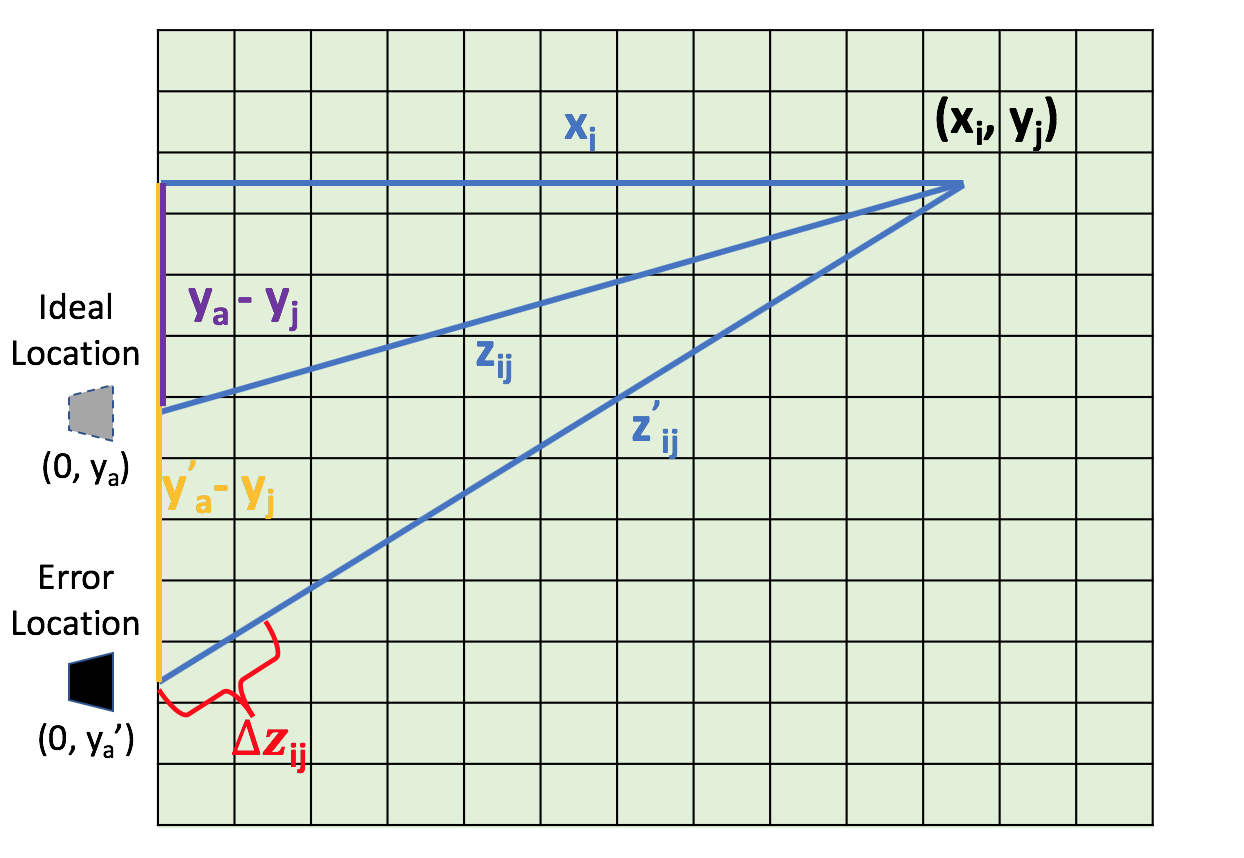
\includegraphics[width=0.4\textwidth]{Figures/PhaseErrMap.png}
\caption{Geometry for phase error calculations.}
\label{PhaseMap}
\end{figure}
\newline
where $k$ is the propagation constant, $\Delta{z}_{ij}$ is defined for each point in the scene, and the factor of two again comes from the two-way propagation. This phase error can be related directly to a time of arrival error for each pixel of the scene. On the other hand, the time of arrival array used in the backprojection algorithm assumes the location of the aperture to be at $u(a)$ rather than $u'(a)$, so it remains unchanged. It is clear that error will exist as values for $s_M(t,u')$, which have incorrect values at the sampled times, are assigned to the pixels. The image can now be expressed as:
\begin{equation}
\label{newIM}
im'(x_i,j_i) = \sum_{u}s'_M(t_{ij}(u),u').
\end{equation}
\begin{figure}[h!]
    \centering
    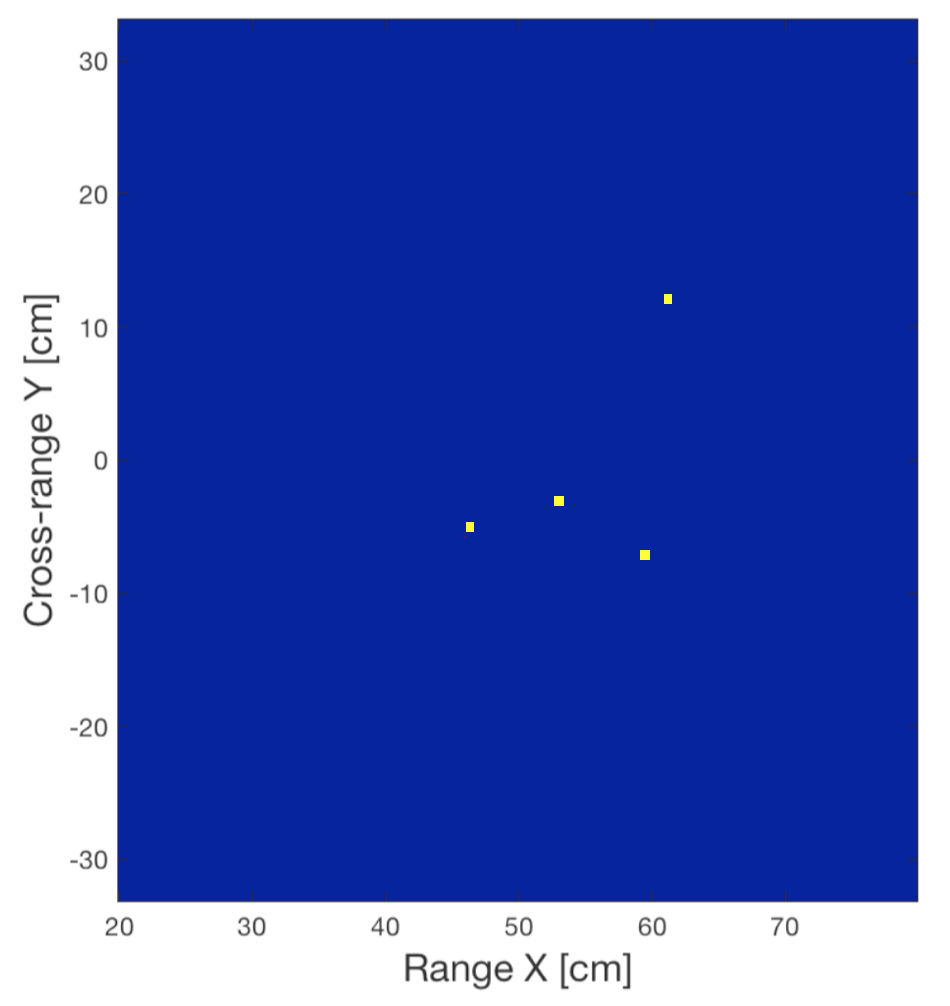
\includegraphics[width=0.35\textwidth]{Figures/TrueTar.png}
\caption{Imaging scene with 4 targets for the MATLAB simulation of aperture location error using the backprojection algorithm.}
\label{TrueTar}
\end{figure}
\indent
To demonstrate the effect of this error in the reconstructed images, we implement location error of the aperture in MATLAB simulations using the backprojection algorithm. The scene being imaged consists of 4 randomly placed targets as seen in Figure \ref{TrueTar}. Other simulation parameters can be found in Table \ref{table:1} above. First, we over-sample the scene at an aperture spacing of $\frac{\lambda}{16}$. To generate the time of arrival array, we use every $8^{th}$ sample, which corresponds to the ideal sampling of $\frac{\lambda}{2}$. For signal capture, we select the samples that correspond to an aperture spacing of $\frac{\lambda}{2} + N(0,\sigma^2)$. The variance is varied over a few different values to show the effect of errors with standard deviation of $\frac{\lambda}{8}$ (500 $\mu$m), $\frac{\lambda}{4}$ (1 mm), and $\frac{\lambda}{2}$ (2 mm) in Figure \ref{ErrorIm}. The reconstructed image with no errors is also shown. As depicted, even with only a 1 mm error in location, the image can no longer provide a meaningful representation of the scene; not only are the targets depicted in invalid locations, but there are several ghost targets that appear. It is clear that this is a practical issue in millimeter-wave radar imaging due to the complexity of knowing the aperture location with sub-millimeter accuracy.
\begin{figure}[h!]
    \centering
    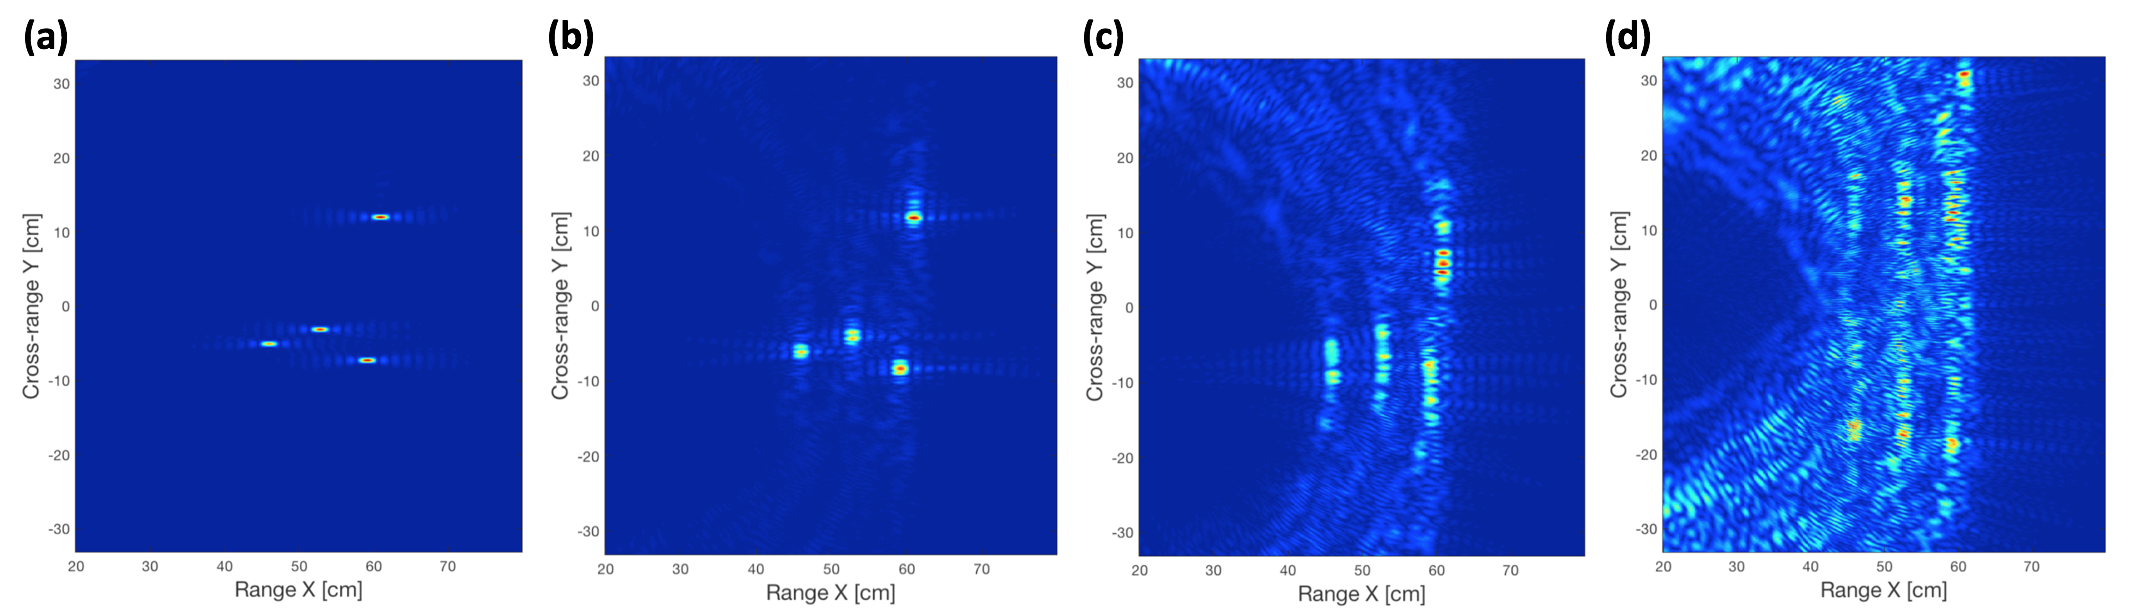
\includegraphics[width=\textwidth]{Figures/ErrorIm2.png}
\caption{Reconstructed image of 4-target scene using back-projection with aperture location errors of (a) $\sigma=0$  ${(no error)}$, (b)   $\sigma=\frac{\lambda}{8}$ (500 $\mu${m}), (c)$ $  $\sigma=\frac{\lambda}{4}$ (1 mm), (d)$ $  $\sigma=\frac{\lambda}{2}$ (2 mm).}
\label{ErrorIm}
\end{figure}
\subsection{Neural Network}
\subsubsection{Introduction}
\indent \indent
As it was demonstrated in previous sections, the effect of phase noise caused by sampling location errors can be significant especially in the case of cumulative errors. Moreover, because of the random nature of the location error in the practical scenarios it is hard to find a linear filter to compensate for the phase noise resulting from location uncertainty. In this section we investigate effect of non-linear filters like convolutional neural nets for mitigation of phase-noise effect in SAR image reconstruction. We first describe the neural network model used as the non-linear phase-error-correction filter. Then we test the neural net model in two different scenarios: the case of iid Gaussian noise in location and cumulative noise in location. 
\subsubsection{Model}
\indent \indent
The neural network used in this project is based on a well known deep learning architecture named convolutional auto-encoders \cite{masci2011stacked}. Auto-encoders consist of compressing/encoding and decompressing/decoding modules that try to map the input data into a robust lower dimensional manifold. This manifold learning can help in learning transforms that are robust to non-idealities of real-world data like phase noise. In case of SAR imaging, the assumption of limited bandwidth of received signal and inherent continuity of radar images captured from natural scenes provides an intuition that natural radar images live on a manifold and as a result a transform that embeds the signal in a low dimensional space might exist that is very robust to location errors. In our project the non-linear transform that transforms the input radar signal to the low dimensional manifold and back consists of 3x3 linear convolution filters, rectified linear unit (relu) activation and pooling layers that try to down sample the input image to achieve a multi-scale transformation between the manifold and the original radar image. Figure \ref{CNN} shows the high-level architecture of the convolutional auto-encoder used in this project.   
\begin{figure}[h!]
    \centering
    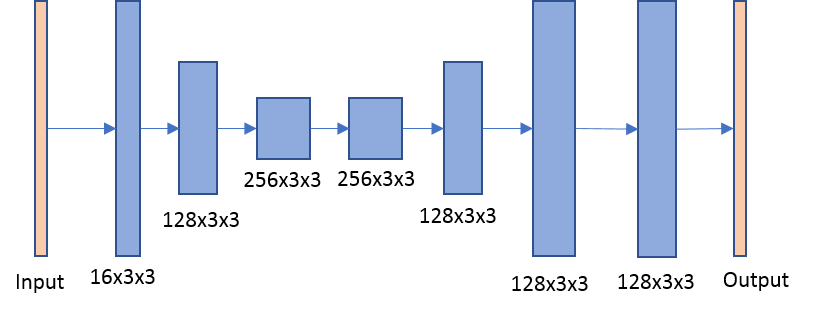
\includegraphics[width=0.845\textwidth]{Figures/CNN.png}
\caption{Convolutional Neural Net architecture}
\label{CNN}
\end{figure}
\newline
\indent
As it can be seen in the figure, the network is designed in a way that it first down-scales the input radar image into a lower dimensional representation and then tries to decode the resulting representation to an image of the same size. In our experiment, the input image is a SAR array time-series with sensor location errors (simulated with an approach similar to the previous sections) and the output is the SAR array time-series data without location error. In other words, the neural network is designed to transform the noisy time-series data into equivalent noiseless signal that can be fed into one of the reconstruction algorithms explained above.
\subsubsection{Experiment design}
In order to insure that the neural net is in fact learning a robust denoising filter and is not memorizing (over-fitting) to the training data and in order to insure an intuitive evaluation of the results, we designed the training and test set in the following way. First, we limited the scene to a single point target with a random position in the field of view but always with the smallest possible size (1 pixel). This helps in estimation of systems resolution by looking at the spread of the reconstructed signal and also helps to make sure the neural network has very slight chance of "memorizing" the location of the target. Moreover we made sure that there are no shared targets between train and test sets. The second important factor that had to be randomized was the SAR array locations. We made sure that the location of each and every training and test sample is randomly generated. Similar to the previous sections we assumed a Gaussian random variable with mean of 8 samples and standard deviation of 4 samples for training. Because of limitation of time and computation resources and in order to accelerate the training of the neural net we limited our training set to iid Gaussian location noise but tested our algorithm on both iid Gaussian and cumulative Gaussian noise. In other words, although the neural net has only seen iid Gaussian noise with standard deviation of 4 samples, it will be tested on both iid noise and cumulative noise that can be modeled as a Gaussian error with increasing variance. 
\subsubsection{Results}
\indent \indent
For the first experiment we first introduce noise in location of each antenna in the SAR array by an iid Gaussian we then feed the resulting signal as a test sample to the neural net. This results in a filtered SAR image that is ready for the SAR image reconstruction using one of the methods explained in the previous sections. Figure \ref{iid_error} shows the image reconstruction artifacts caused by the location error with and without neural net filtering. This figure is generated by subtracting the reconstructed SAR image with location noise from similar image without any noise. We used the back-projection algorithm for reconstruction of all of the SAR images. 
\begin{figure}[h!]
    \centering
    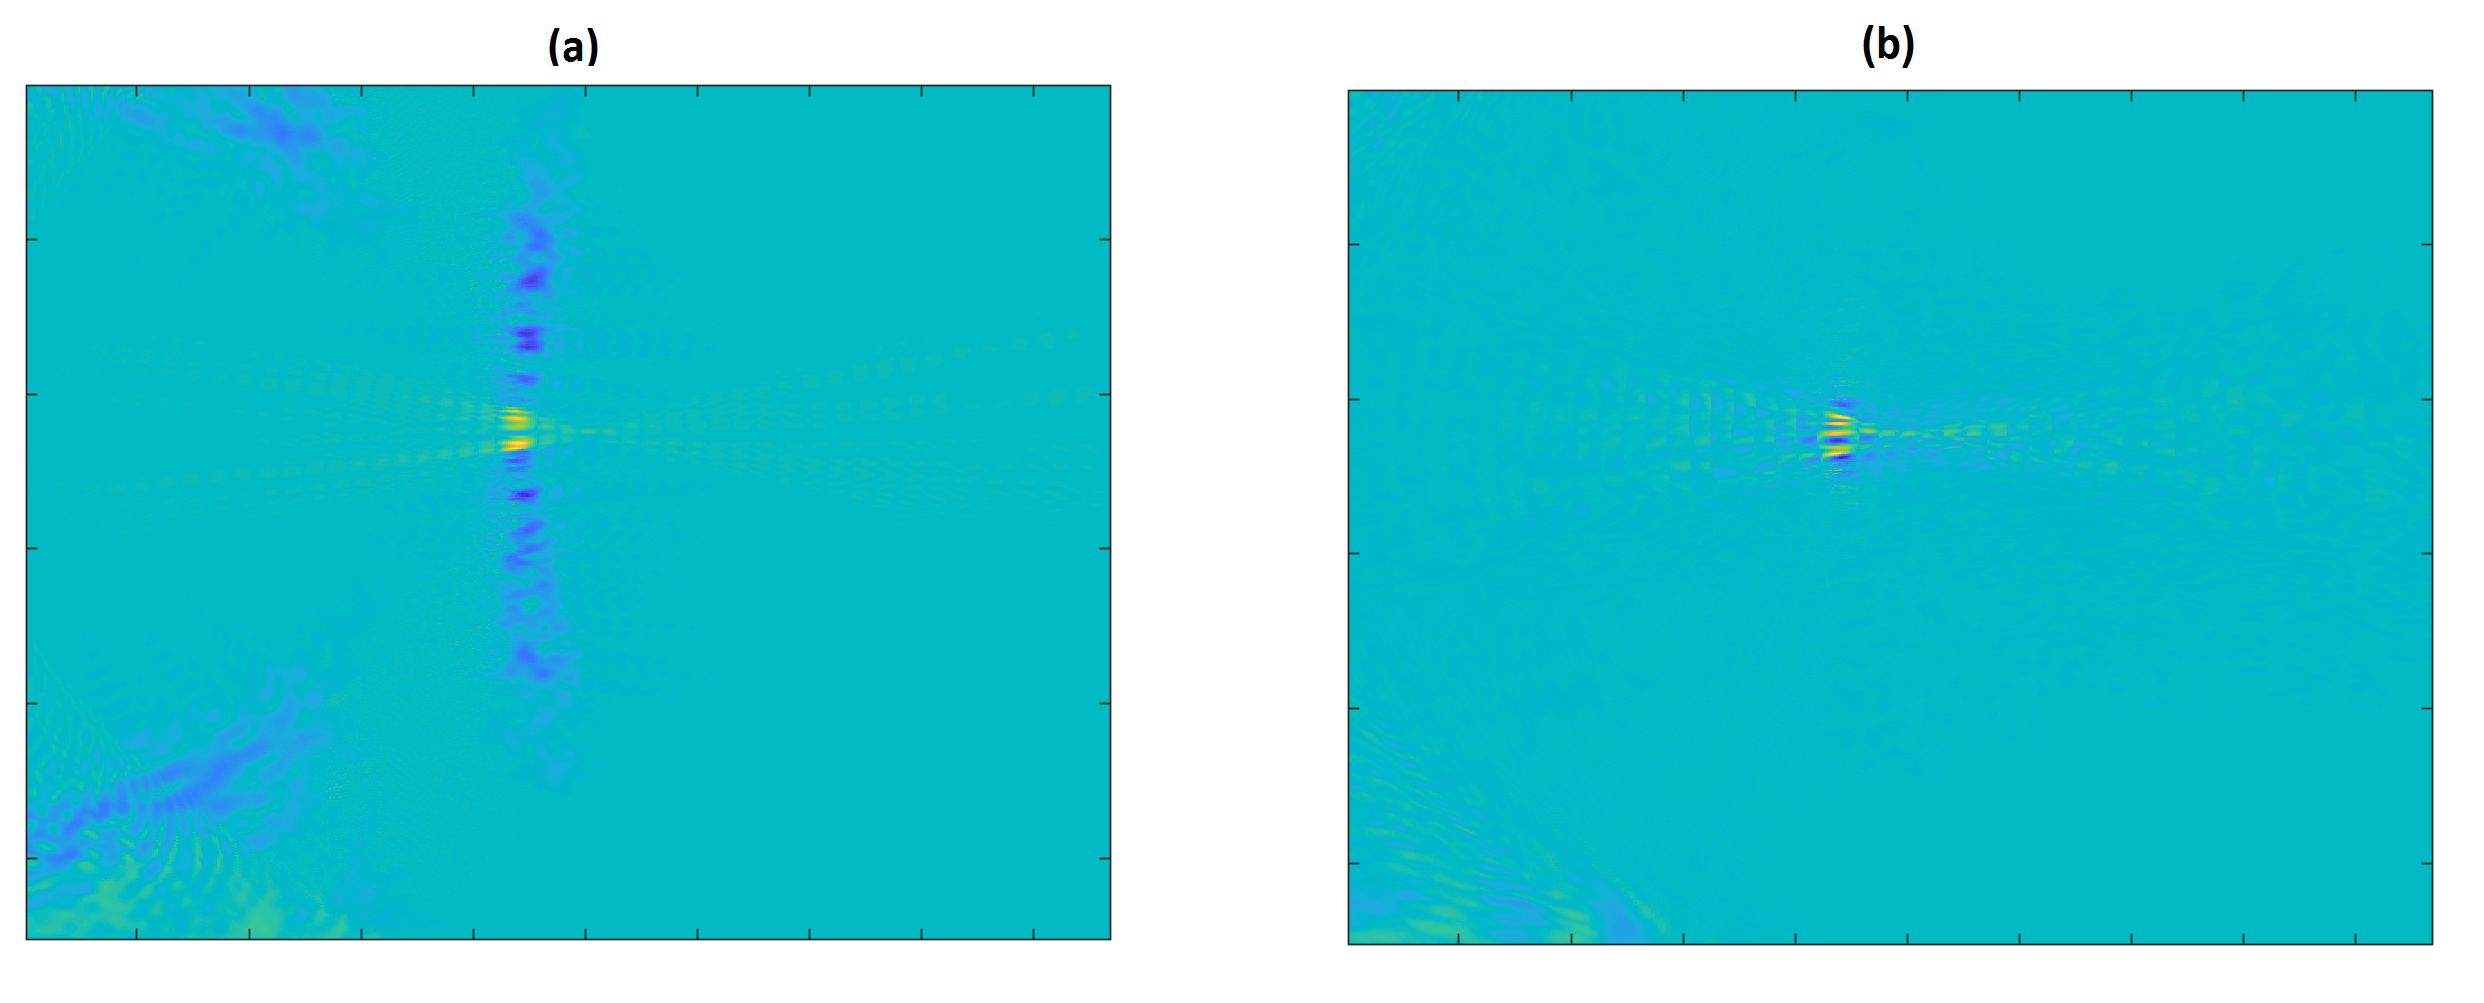
\includegraphics[width=0.845\textwidth]{Figures/linear_nn_vs_no_nn.png}
\caption{Artifacts caused by iid Gaussian location error . (a) Artifacts in reconstructed SAR image caused by iid error without filtering. (b) Artifacts in reconstructed SAR image caused by iid error after CNN filtering.}
\label{iid_error}
\end{figure}
\newline
\indent
As it can be seen, the phase noise causes the SAR algorithm to elongate the target in the direction of the aperture (cross-range). However, it can be seen in figure \ref{iid_error} (b) that the neural net successfully has captured the effect of the phase noise and has compensated for it.
For the second experiment we modeled the SAR array location error as a cumulative Gaussian process. It should be mentioned that the neural network was not retrained for this experiment and is completely unaware of the different location error distribution. The result of this experiment can be seen in figure \ref{cumsum_error}.

\begin{figure}[h!]
    \centering
    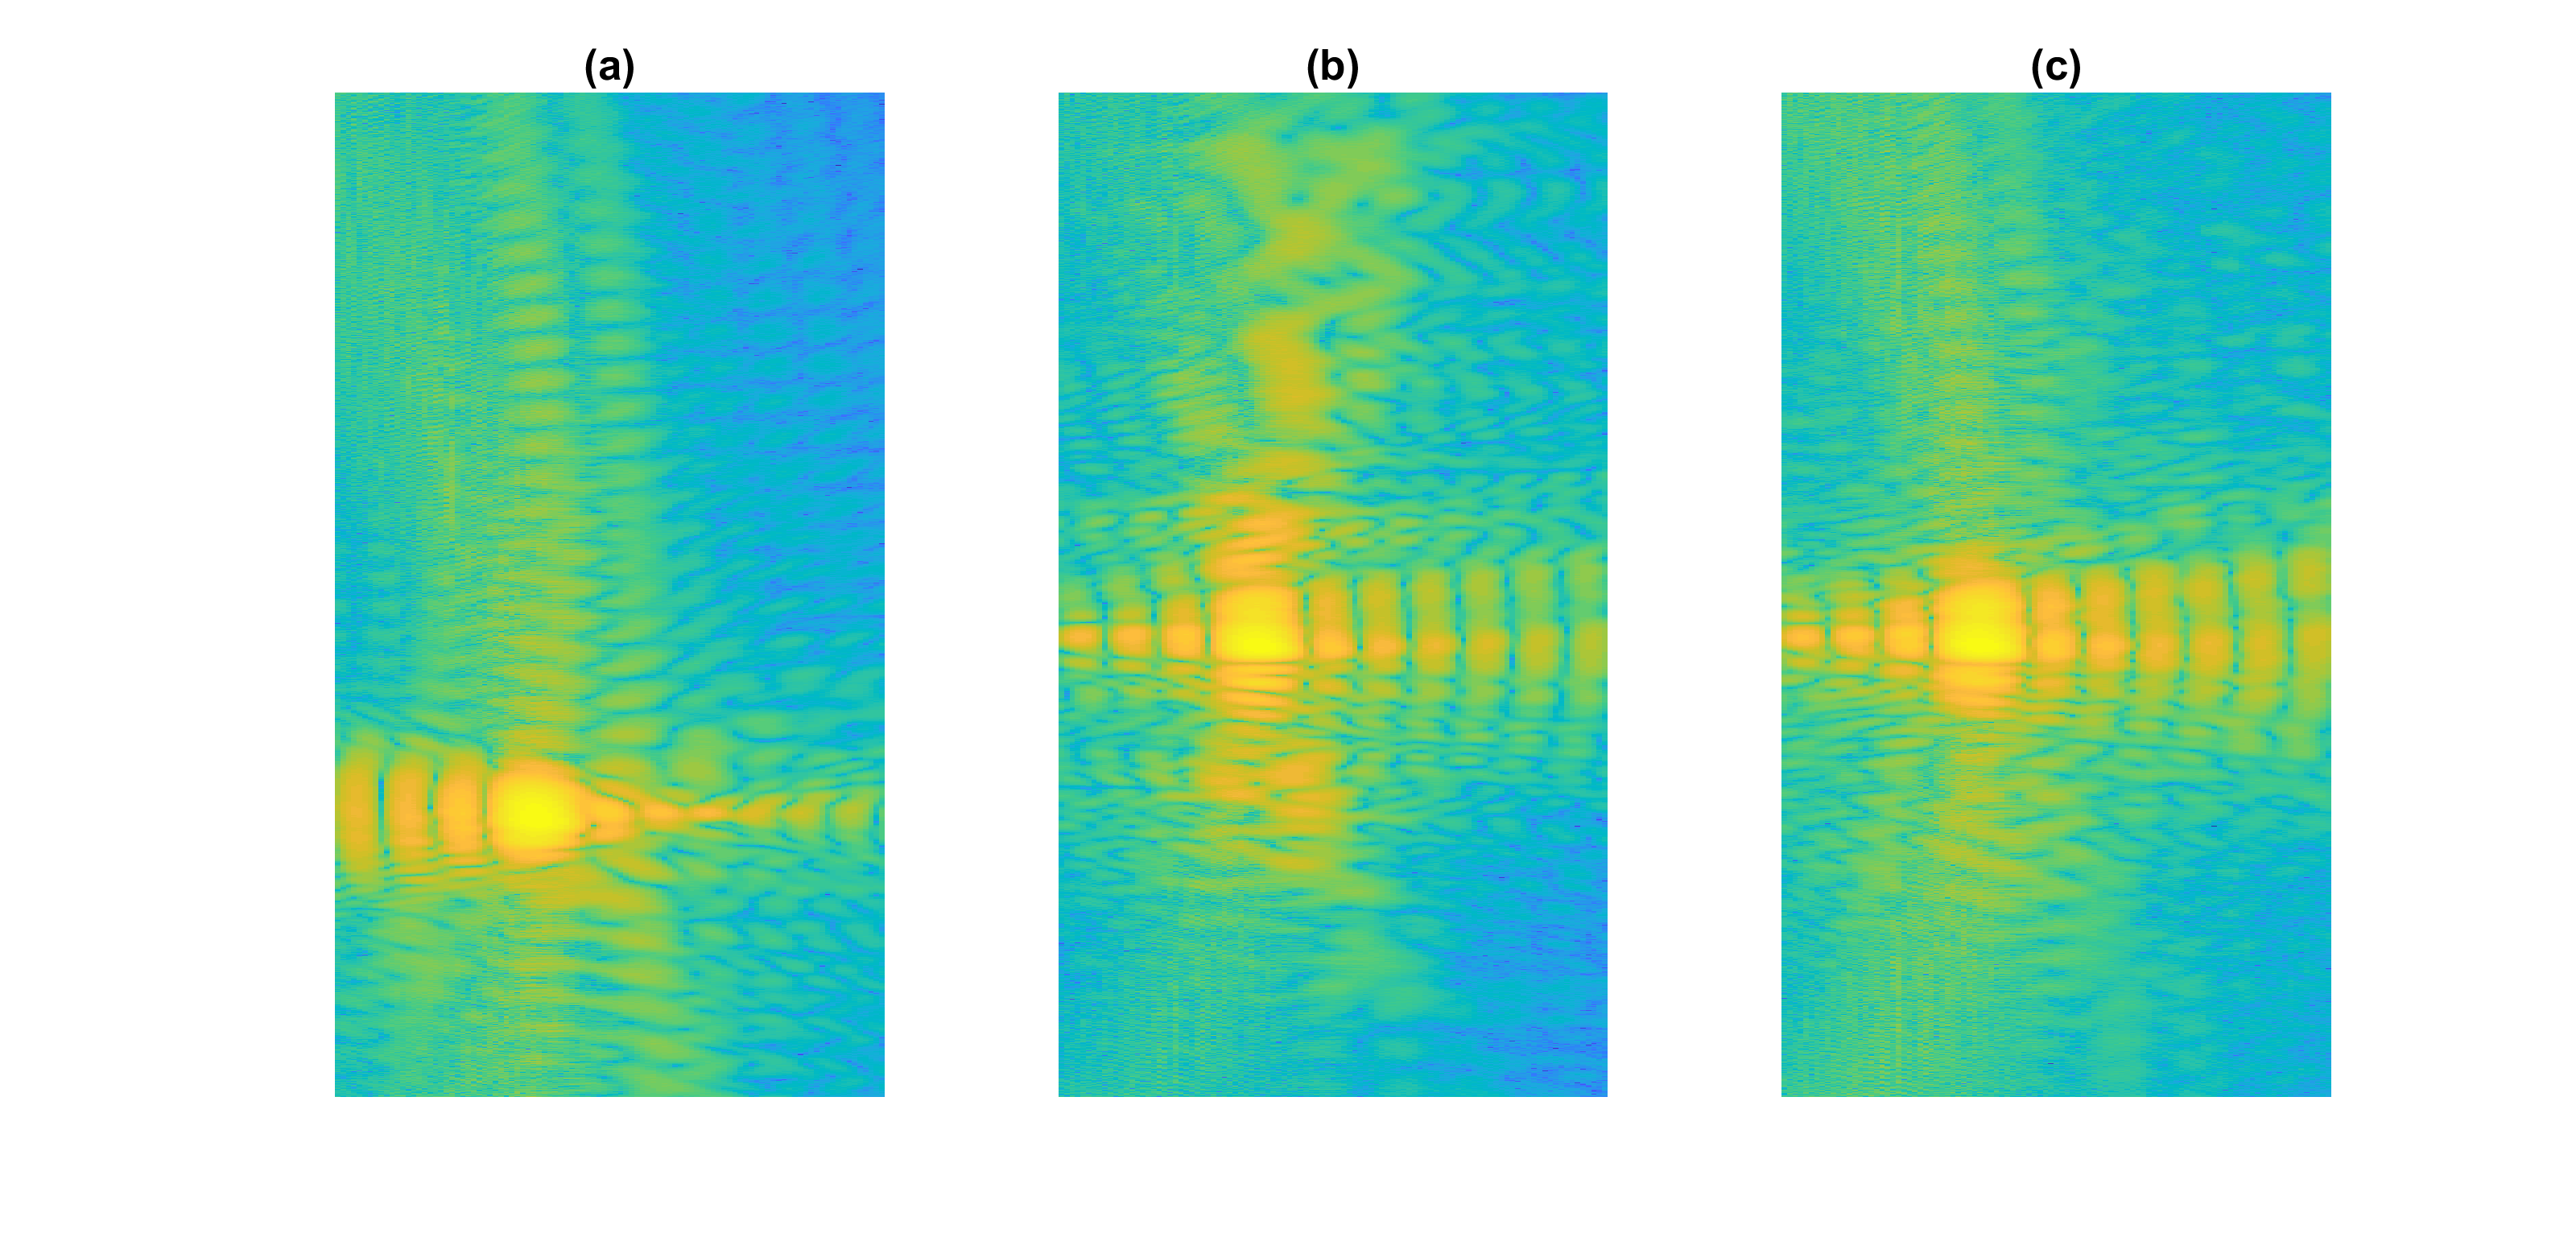
\includegraphics[width=0.945\textwidth]{Figures/zoomed_nl.png}
\caption{Artifacts caused by cumulative Gaussian error. (a) Reconstructed SAR image with no location error. (b) Reconstructed image in case of cumulative Gaussian error without filtering. (c) Reconstructed image after CNN filtering.}
\label{cumsum_error}
\end{figure}
A comparison between (a) and (b) in figure \ref{cumsum_error} shows that the cumulative error has two distinct effects: spreading the point function across cross-range, and a shift of the point target in the direction of accumulation (direction of movement). A comparison between the neural-net-filtered result (c) in the same figure shows that the neural net has successfully reduced the point spread in the cross-range direction. However, the neural net failed to compensate for the shift artifact. This might be caused by the fact that the neural net expects an iid location error distribution. In future work, it would be interesting to see if the neural network would be able to also compensate for this effect.  

\section{Summary and Conclusion}
In this project we first investigated three of the well-known algorithms used in Synthetic Aperture Radar image Reconstruction. Then we elaborated on the effect of location error on these algorithms through both theoretical and experimental (simulated) analysis. We observed that in case of mmWave SAR imaging systems, small errors (in range of a few millimeters) in location of each imaging element can have a drastic effect on the imaging resolution and this effect is amplified if the error is cumulative in nature, which is the case in most IMU-based localization systems. We observed that the effect of this error is very dependant on the image reconstruction algorithm which makes it hard to come up with a general solution to artifacts caused by the location error. As the final step in our analysis, we investigated applications of non-linear neural-net-based filters in mitigation of the mentioned artifacts. The results show that neural nets can be very effective in reducing the cross-range spread artifacts caused by location error. However, other more advanced effects like shifting artifacts are still an issue. We observed this type of artifacts in our simulations specially for accumulative error experiments. Compensation for this type of artifacts requires design of a more advanced non-linear filter that will be the direction of future work in this area. 
\section{Appendix}
\indent \indent
This appendix comments on the MATLAB code that was used for the two reconstruction algorithms. It originates from \cite{SARbook}; however, we have edited it to fit the application of a millimeter-wave radar, to randomize the location of the targets, as well as to introduce random location errors. The relevant algorithms to our report are the 2D Matched Filtering and Interpolation and the Backprojection algorithm; however, most of the code plays a role in initializing critical parameters. The code has been appended to the end of this document.

\nocite{*}
\bibliography{ref.bib}
\bibliographystyle{IEEEtran}

\end{document}
